%%%%%%%%%%%%%%%%%%%%%%%%%%%%%%%%%%%%%%%%%%%%%%%%%%%%%%%%%%%%%%%%%%%%%%%%%%%%%%%%%%%%%%%%%%%%%%%%%%%%%%%%%%%%%%%%%%%%%%%%%%%%%%%%%%%%%%%%%%%%%%%%%%%%%%%%%%%

%%%%%%%%%%%%%%%%%%%%%%%%%%%%%%%%%%%%%%%%%%%%%%%%%%%%%%%%%%%%%%%%%%%%%%%%%%%%%%%%%%%%%%%%%%%%%%%%%%%%%%%%%%%%%%%%%%%%%%%%%%%%%%%%%%%%%%%%%%%%%%%%%%%%%%%%%%%
% This is just an example/guide for you to refer to when producing your supplementary material for your Frontiers article.                                 %
%%%%%%%%%%%%%%%%%%%%%%%%%%%%%%%%%%%%%%%%%%%%%%%%%%%%%%%%%%%%%%%%%%%%%%%%%%%%%%%%%%%%%%%%%%%%%%%%%%%%%%%%%%%%%%%%%%%%%%%%%%%%%%%%%%%%%%%%%%%%%%%%%%%%%%%%%%%

%%% Version 2.5 Generated 2018/06/15 %%%
%%% You will need to have the following packages installed: datetime, fmtcount, etoolbox, fcprefix, which are normally inlcuded in WinEdt. %%%
%%% In http://www.ctan.org/ you can find the packages and how to install them, if necessary. %%%
%%%  NB logo1.jpg is required in the path in order to correctly compile front page header %%%

\documentclass[utf8]{frontiers_suppmat} % for all articles
\usepackage{url,hyperref,lineno,microtype}
\usepackage[onehalfspacing]{setspace}
\usepackage{lscape} 
\usepackage{cleveref}

% Leave a blank line between paragraphs instead of using \\

\begin{document}
\onecolumn
\firstpage{1}

\title[Supplementary Material]{{\helveticaitalic{Supplementary Material}}}

\maketitle

\section{Supplementary Data}
\begin{itemize}
    \item \textbf{Data Sheet 1.} Gene and pathways associated with each osmolyte included in this study. For each compound, the type of reaction, named reaction type, reaction number, enzyme number, and KEGG ortholog are detailed, as well as the the pathway and step in each pathway that were manually annotated for this study. 
    \item \textbf{Data Sheet 2.} KEGG ortholog presence and absence for each of the reference genomes from MarRef and transcriptomes within the MMETSP. 
    \item \textbf{Data Sheet 3.} Predicted synthesis, breakdown, and transport of each metabolite for each of the reference genomes from MarRef and transcriptomes from MMETSP.
    \item \textbf{Data Sheet 4.} The HMM bitscore thresholds for each KEGG ortholog used in the analysis of recovered Tara orthologs from OM-RGC v2 and MATOU v1. The number of orthologs returned from Ocean Gene Atlas are reported (with an e-value cutoff of 1e-10). The orthologs that pass the HMM bitscore threshold were included in the presented analysis. 
    
\end{itemize}
\section{Supplementary Figures}

\begin{figure*}[ht]
    \centering
    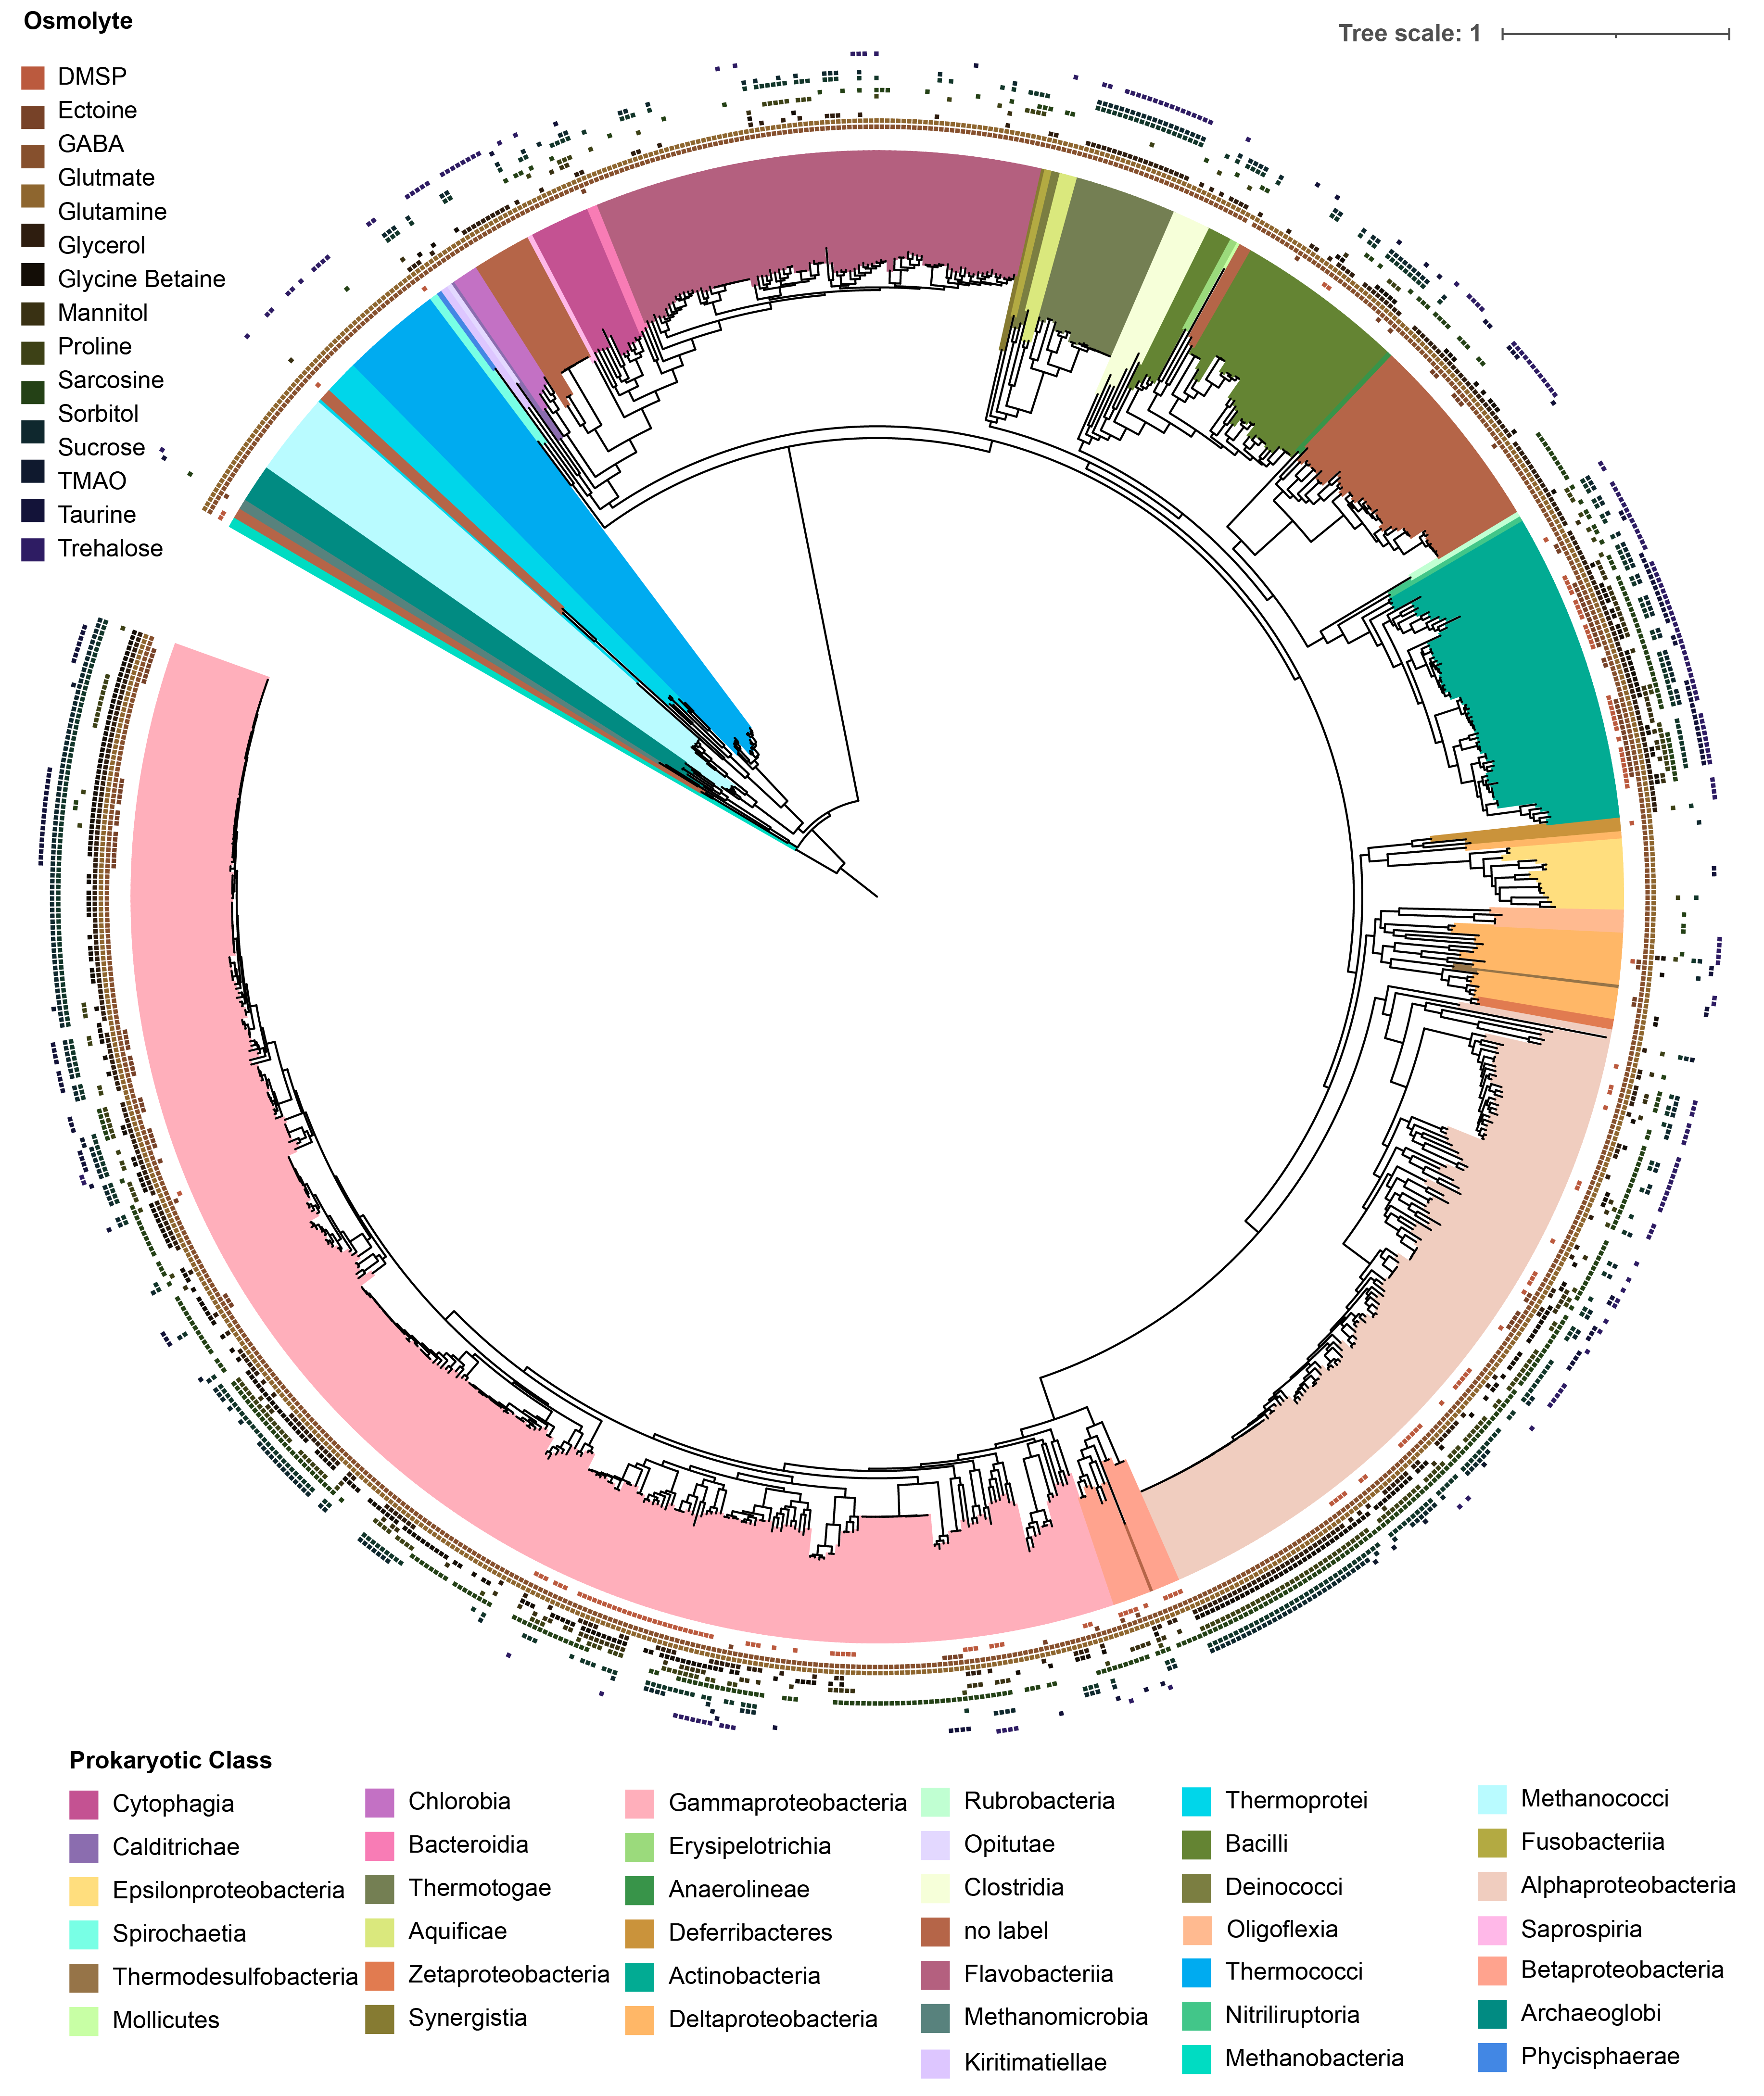
\includegraphics[width=0.9\columnwidth]{Figures/SI-Bacterial-Phylogeny-Synthesis-01-01.png}
    \caption{Maximum likelihood phylogeny of the MarRef genomes depicting synthesis of osmolytes of interest. The concatenated gene tree was constructed using the `Universal` dataset of 15 genes as defined by Hug et al. (2016) and default parameters within GToTree. The presence or absence of the ability to synthesis of each of the osmolytes is depicted for each genome.
}
    \label{fig:physyn}
\end{figure*}

\begin{figure*}
    \centering
    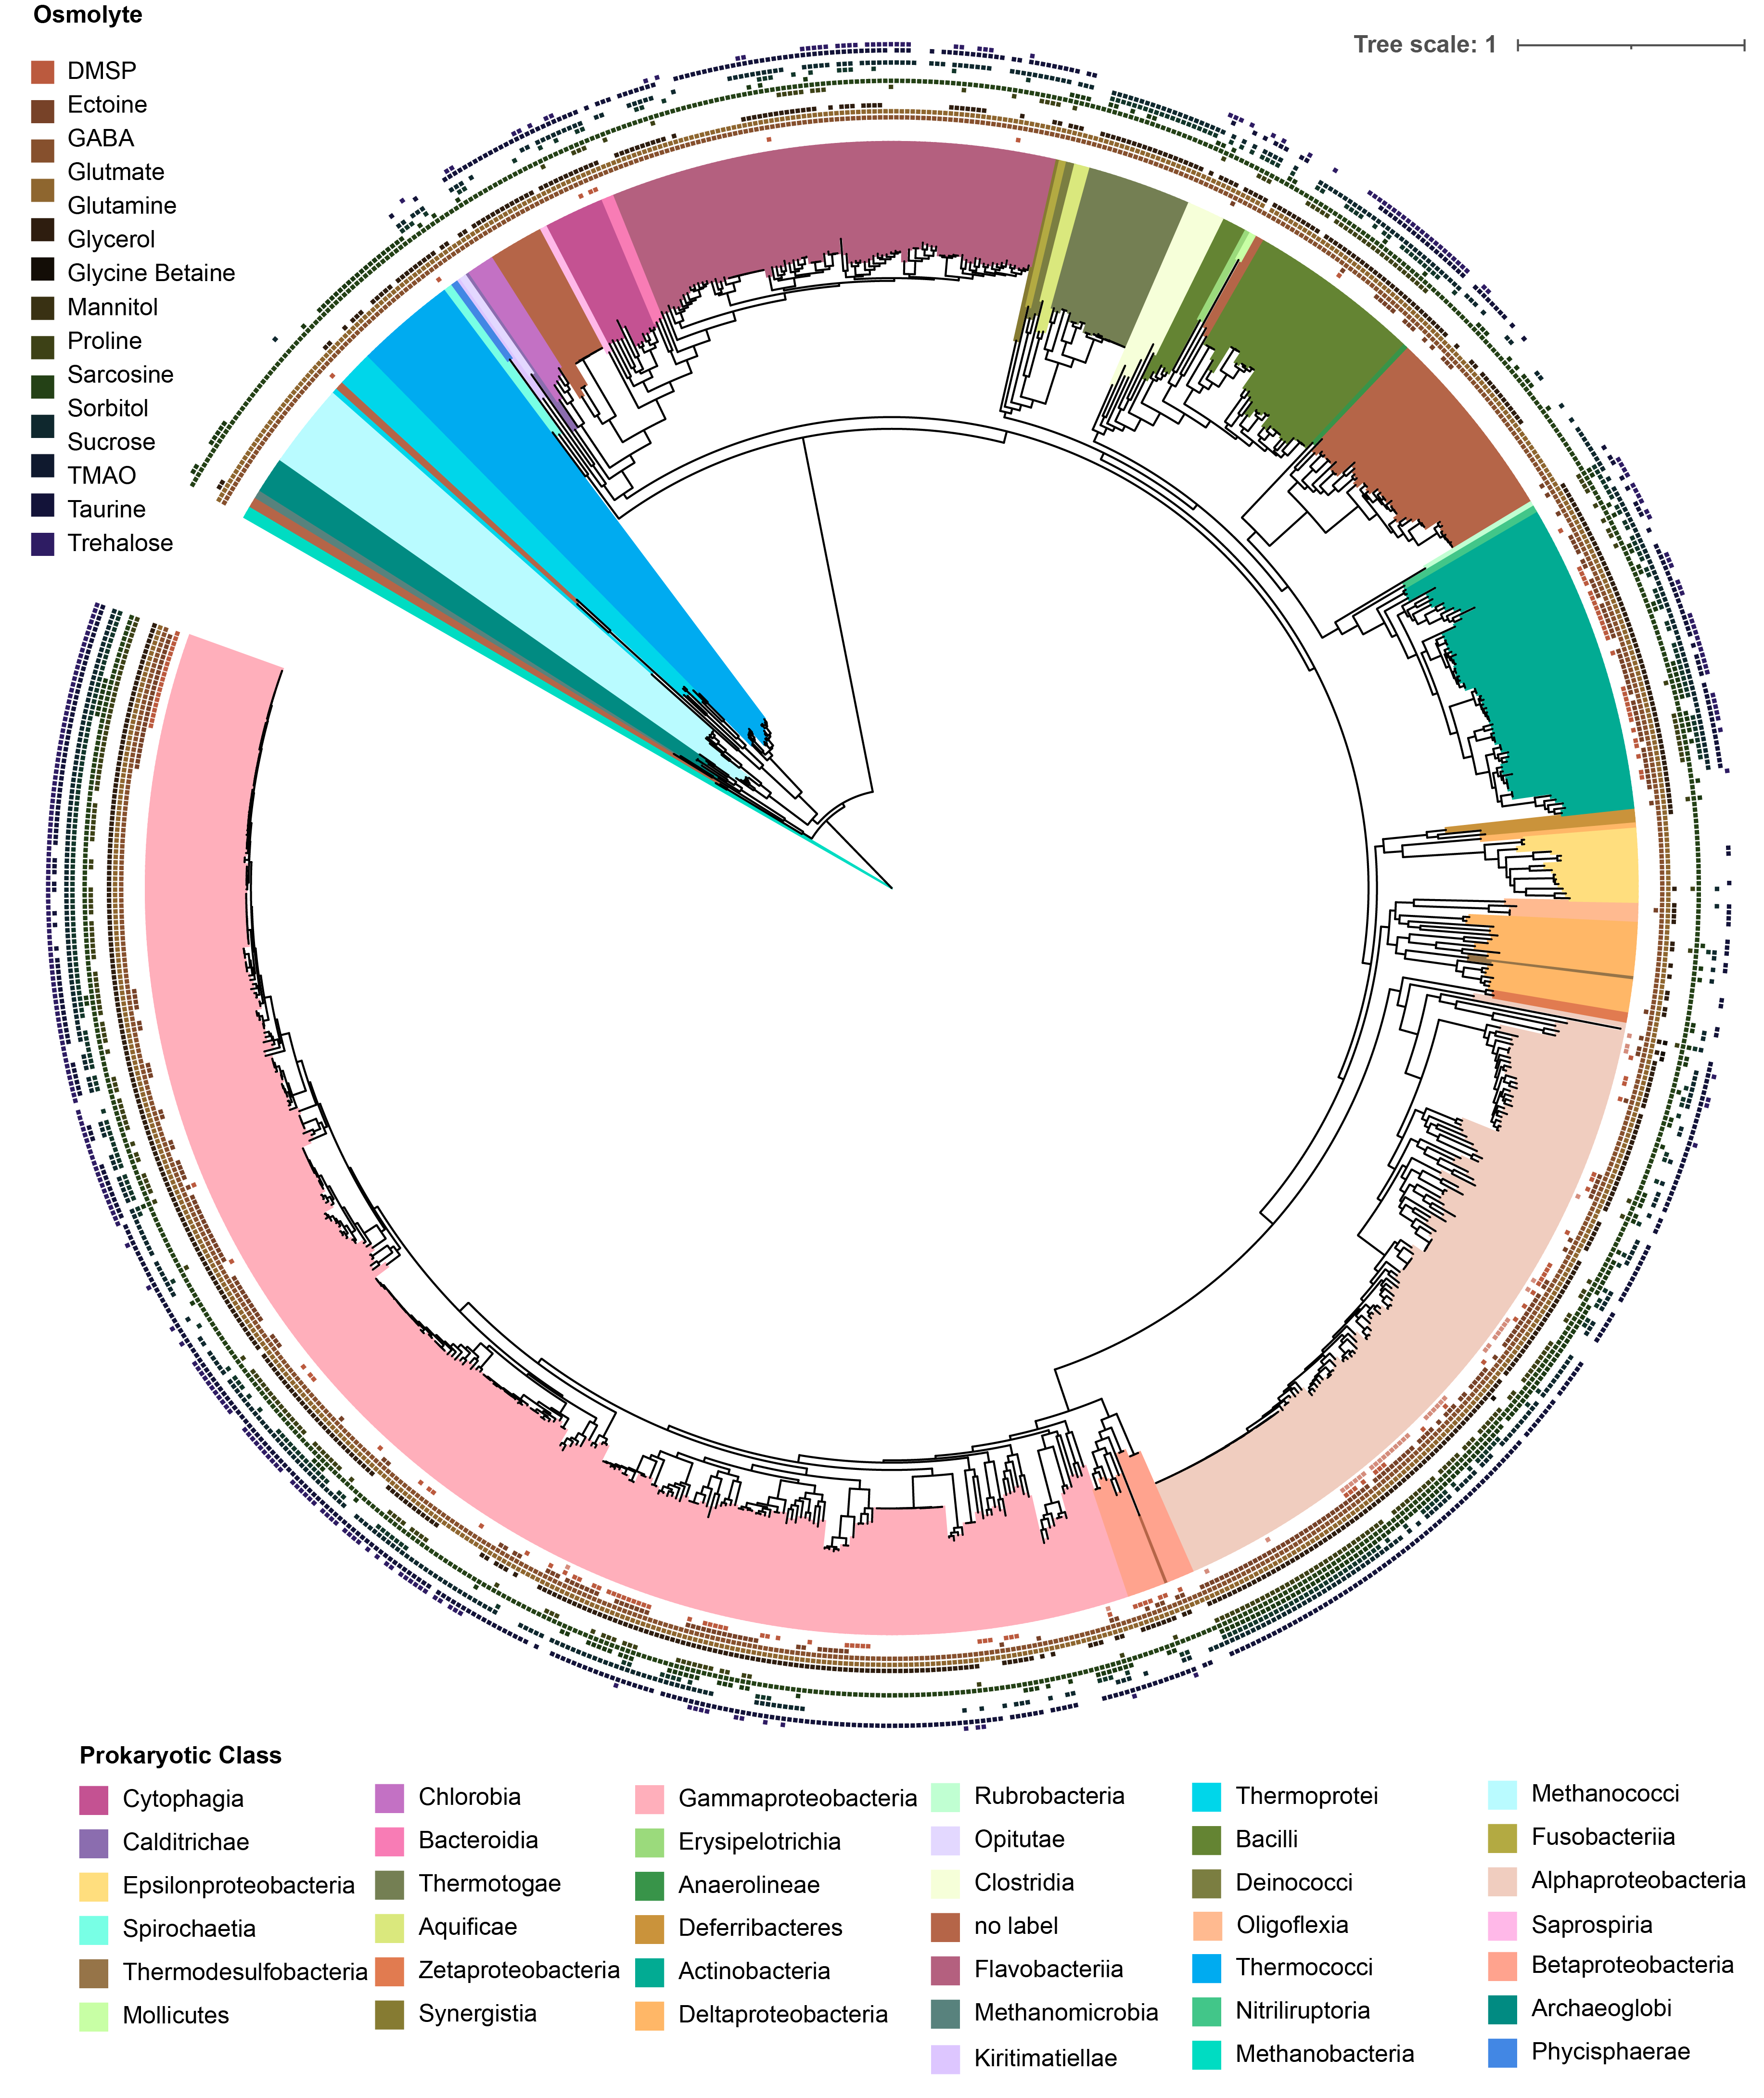
\includegraphics[width=0.9\columnwidth]{Figures/SI-Bacterial-Phylogeny-Breakdown-01-01.png}
    \caption{Maximum likelihood phylogeny of the MarRef genomes depicting breakdown of osmolytes of interst. The concatenated gene tree was constructed using the `Universal` dataset of 15 genes as defined by Hug et al. (2016) and default parameters within GToTree. The presence or absence of the ability to breakdown of each of the osmolytes is depicted for each genome.
}
    \label{fig:phybd}
\end{figure*}

\begin{figure*}[ht]
    \centering
    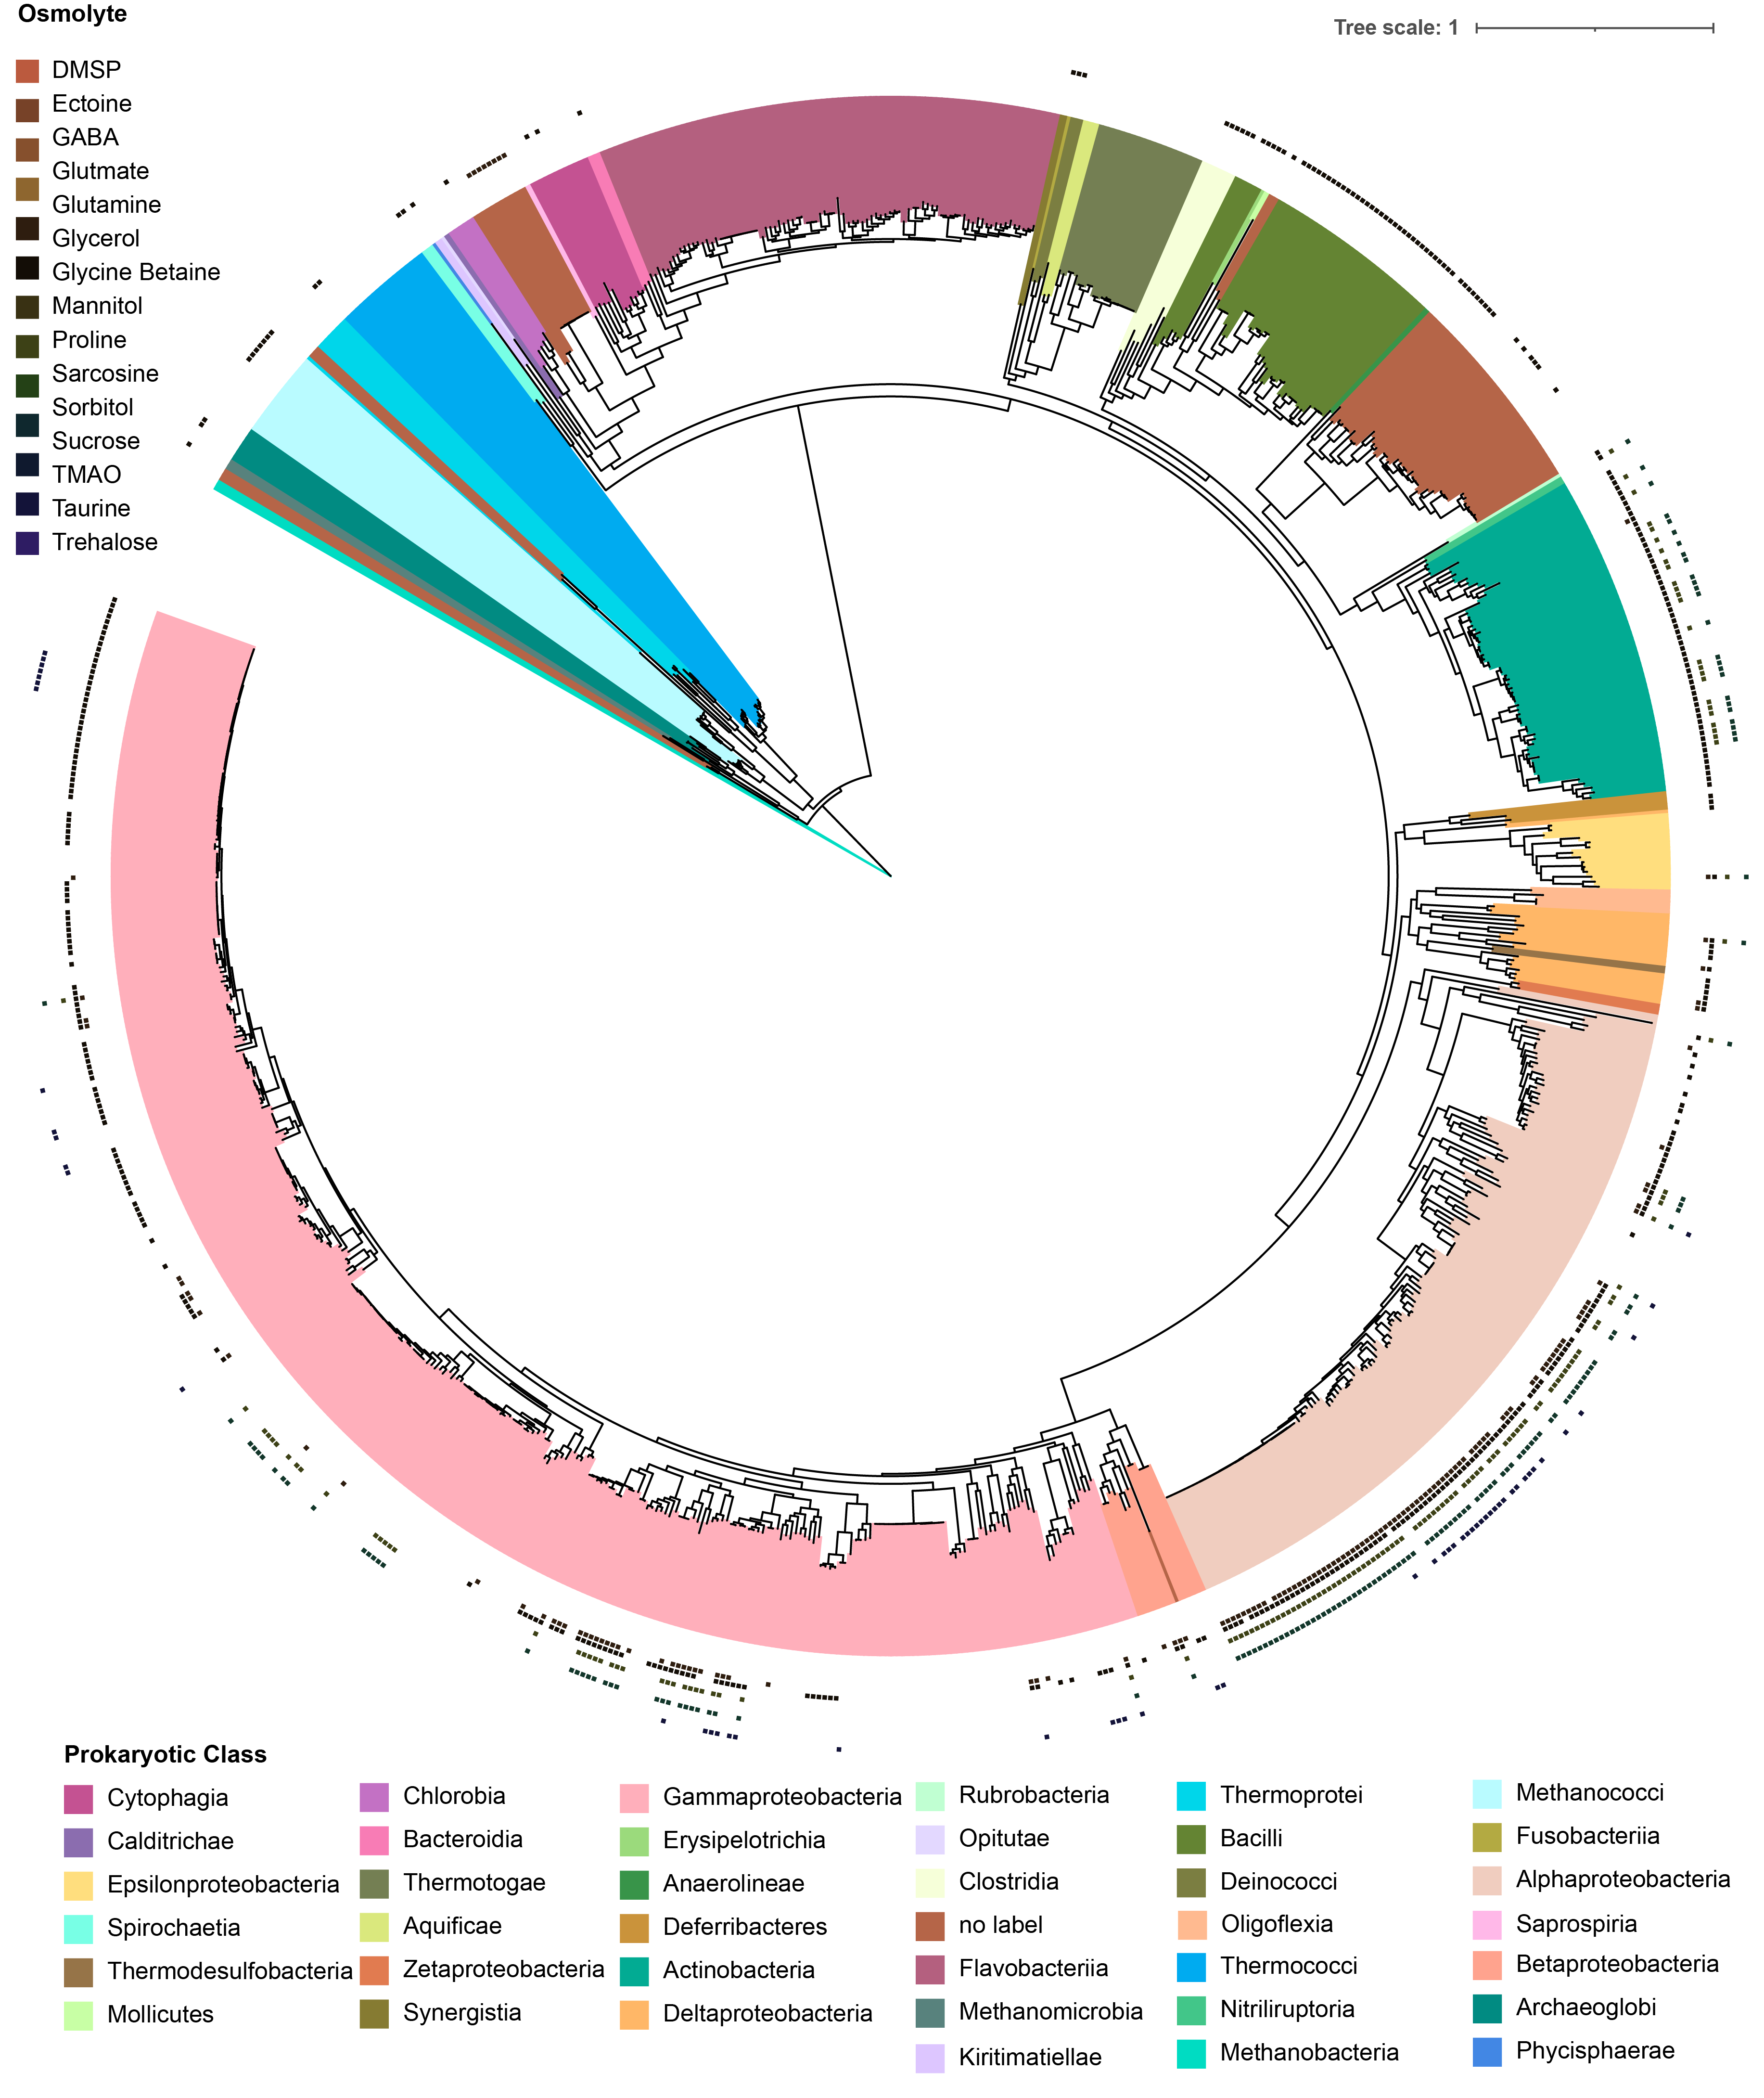
\includegraphics[width=0.9\columnwidth]{Figures/SI-Bacterial-Phylogeny-Transport-01-01.png}
    \caption{Maximum likelihood phylogeny of the MarRef genomes depicting transport of osmolytes of interest. The concatenated gene tree was constructed using the `Universal` dataset of 15 genes as defined by Hug et al. (2016) and default parameters within GToTree. The presence or absence of the ability to transport of each of the osmolytes is depicted for each genome.
}
    \label{fig:phytrans}
\end{figure*}

\begin{figure*}[ht]
    \centering
    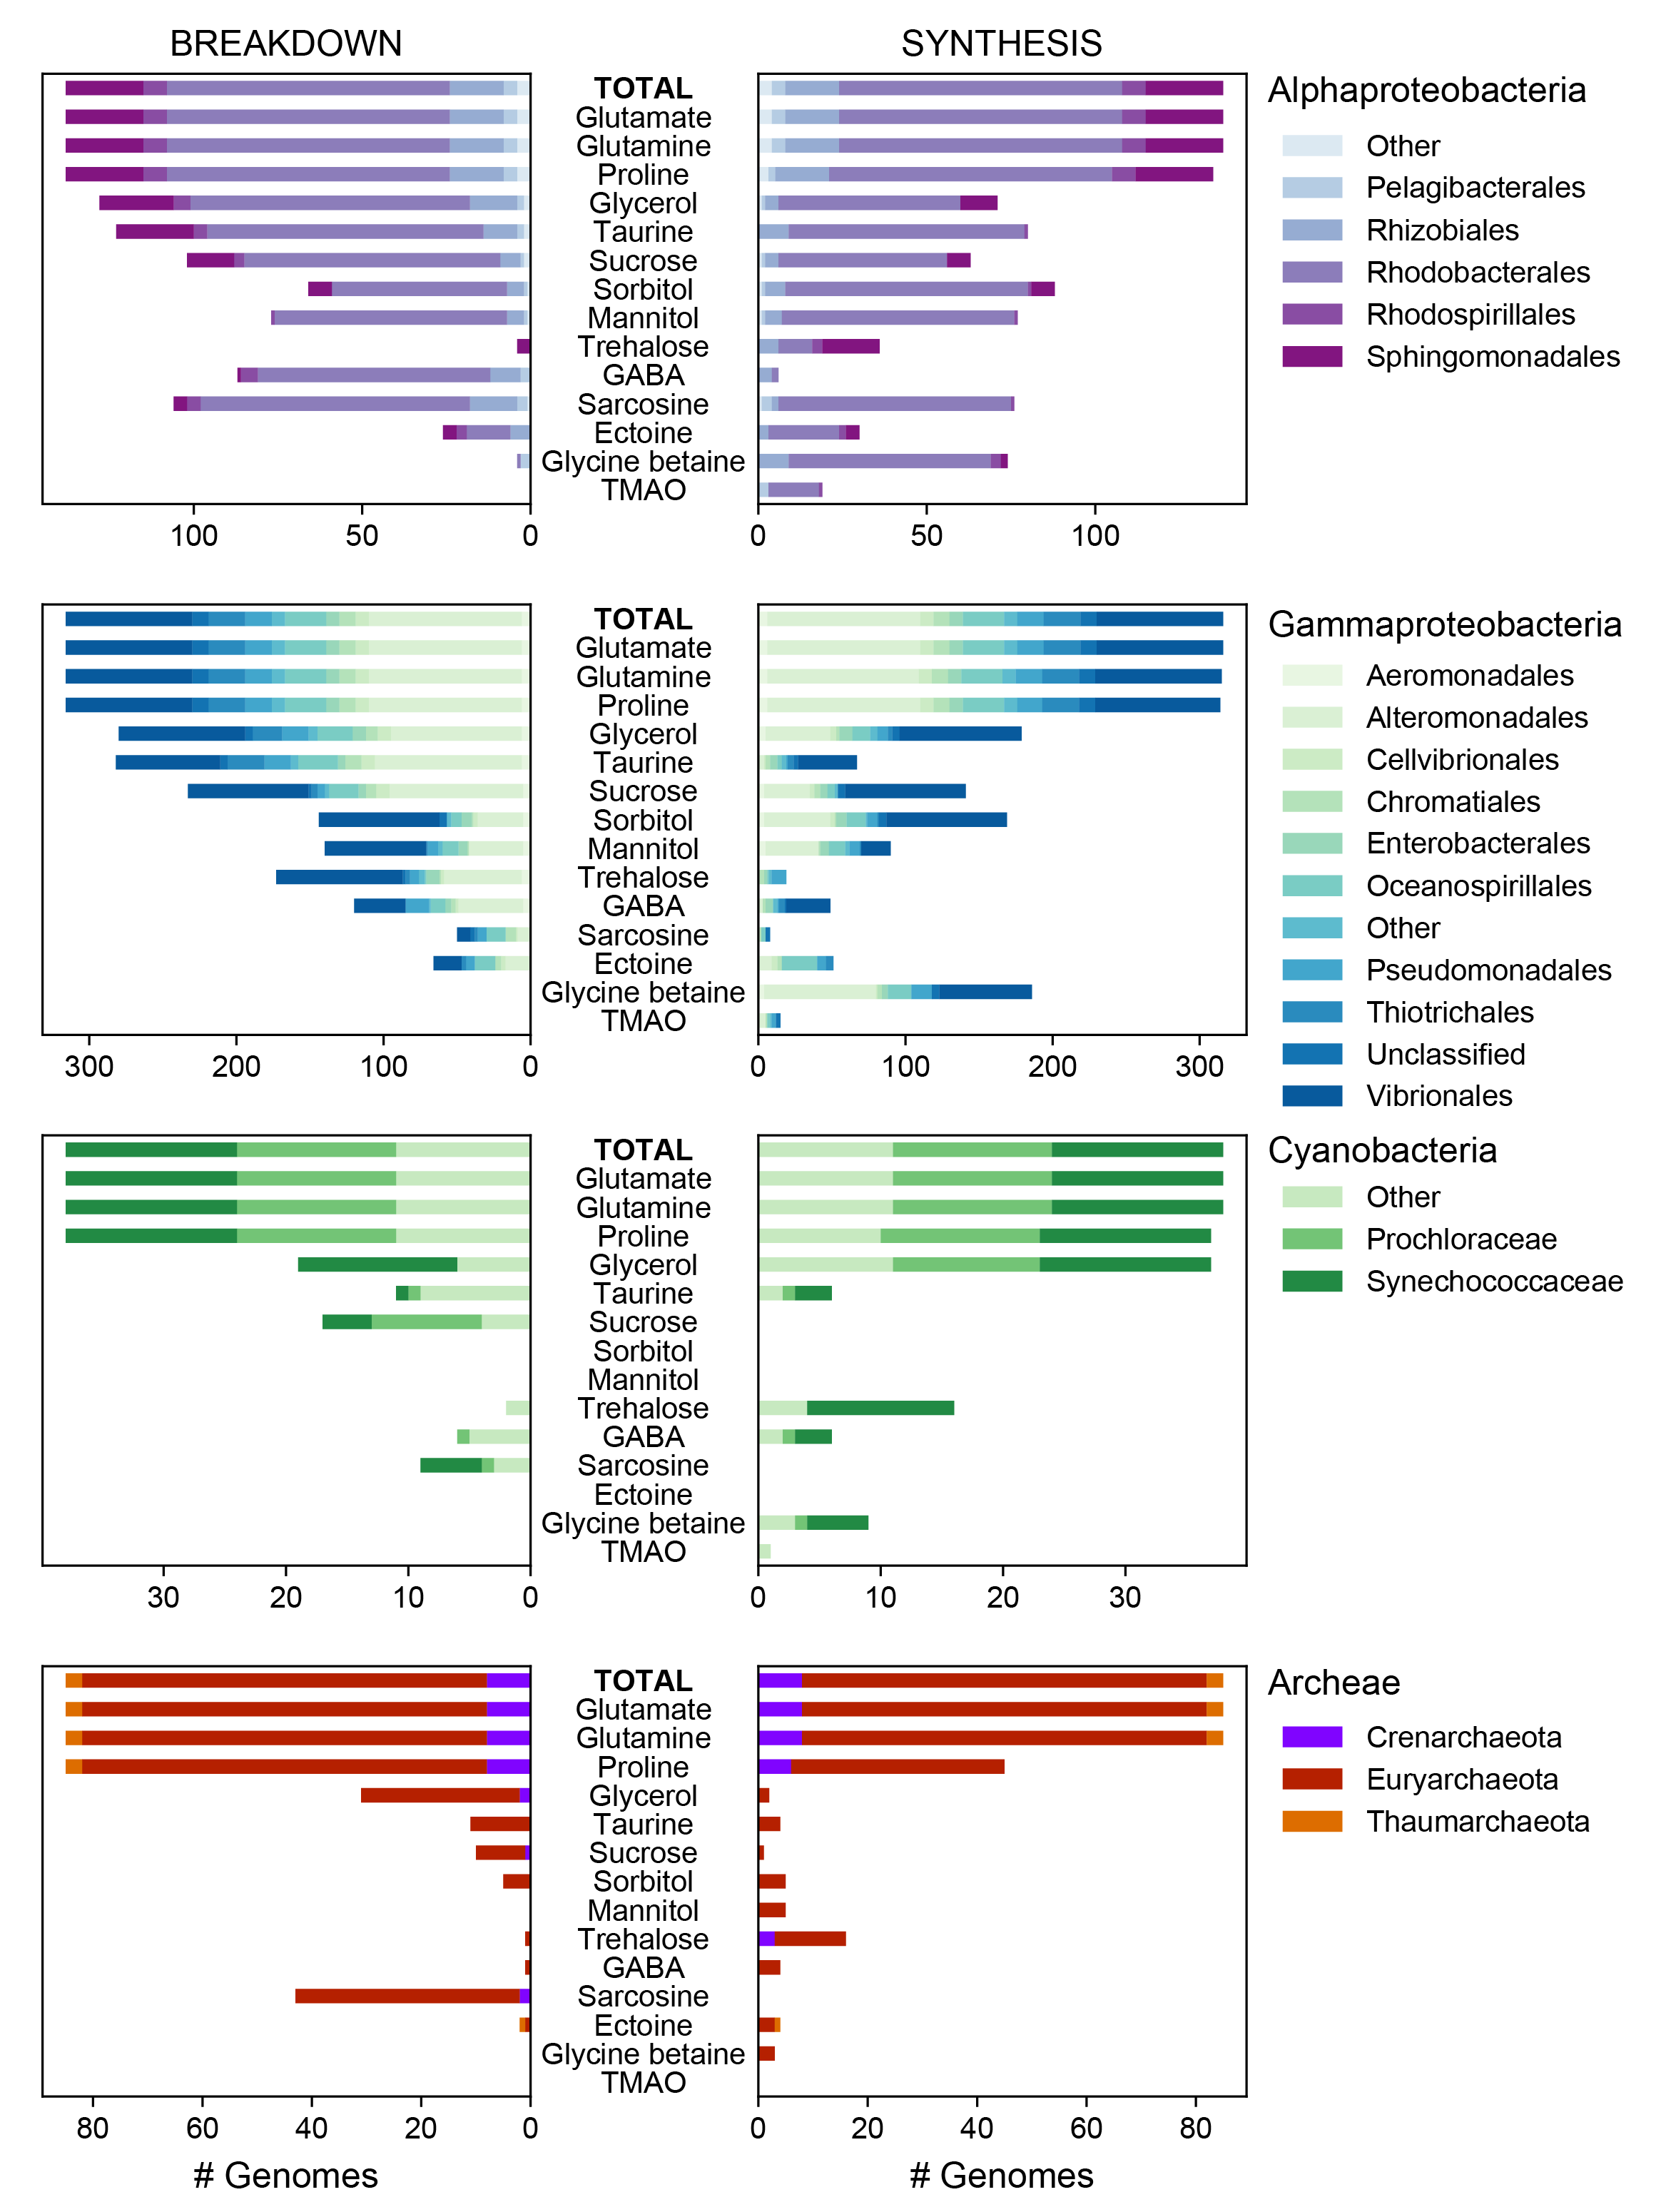
\includegraphics[width=0.9\columnwidth]{Figures/SI-Groups-Syn_BD-01.png}
    \caption{The predicted synthesis and breakdown of targeted osmolytes four major subgroups of prokaryotes shown in (Figure 1): Alphaproteobacteria, Gammaproteobacteria, Cyanobacteria, and Archeae. The breakdown and synthesis of osmolytes within these groups is depicted as a stacked bar graph, and is colored by the designated taxonomic order for Alpha- and Gammaproteobacteria, family for Cyanobacteria, and phylum for Archeae. Osmolytes are sorted along the y-axis based on the total number of genomes capable of breaking down a given osmolyte as in (Figure 1).}
    \label{fig:groups}
\end{figure*}


\begin{figure*}[ht]
    \centering
    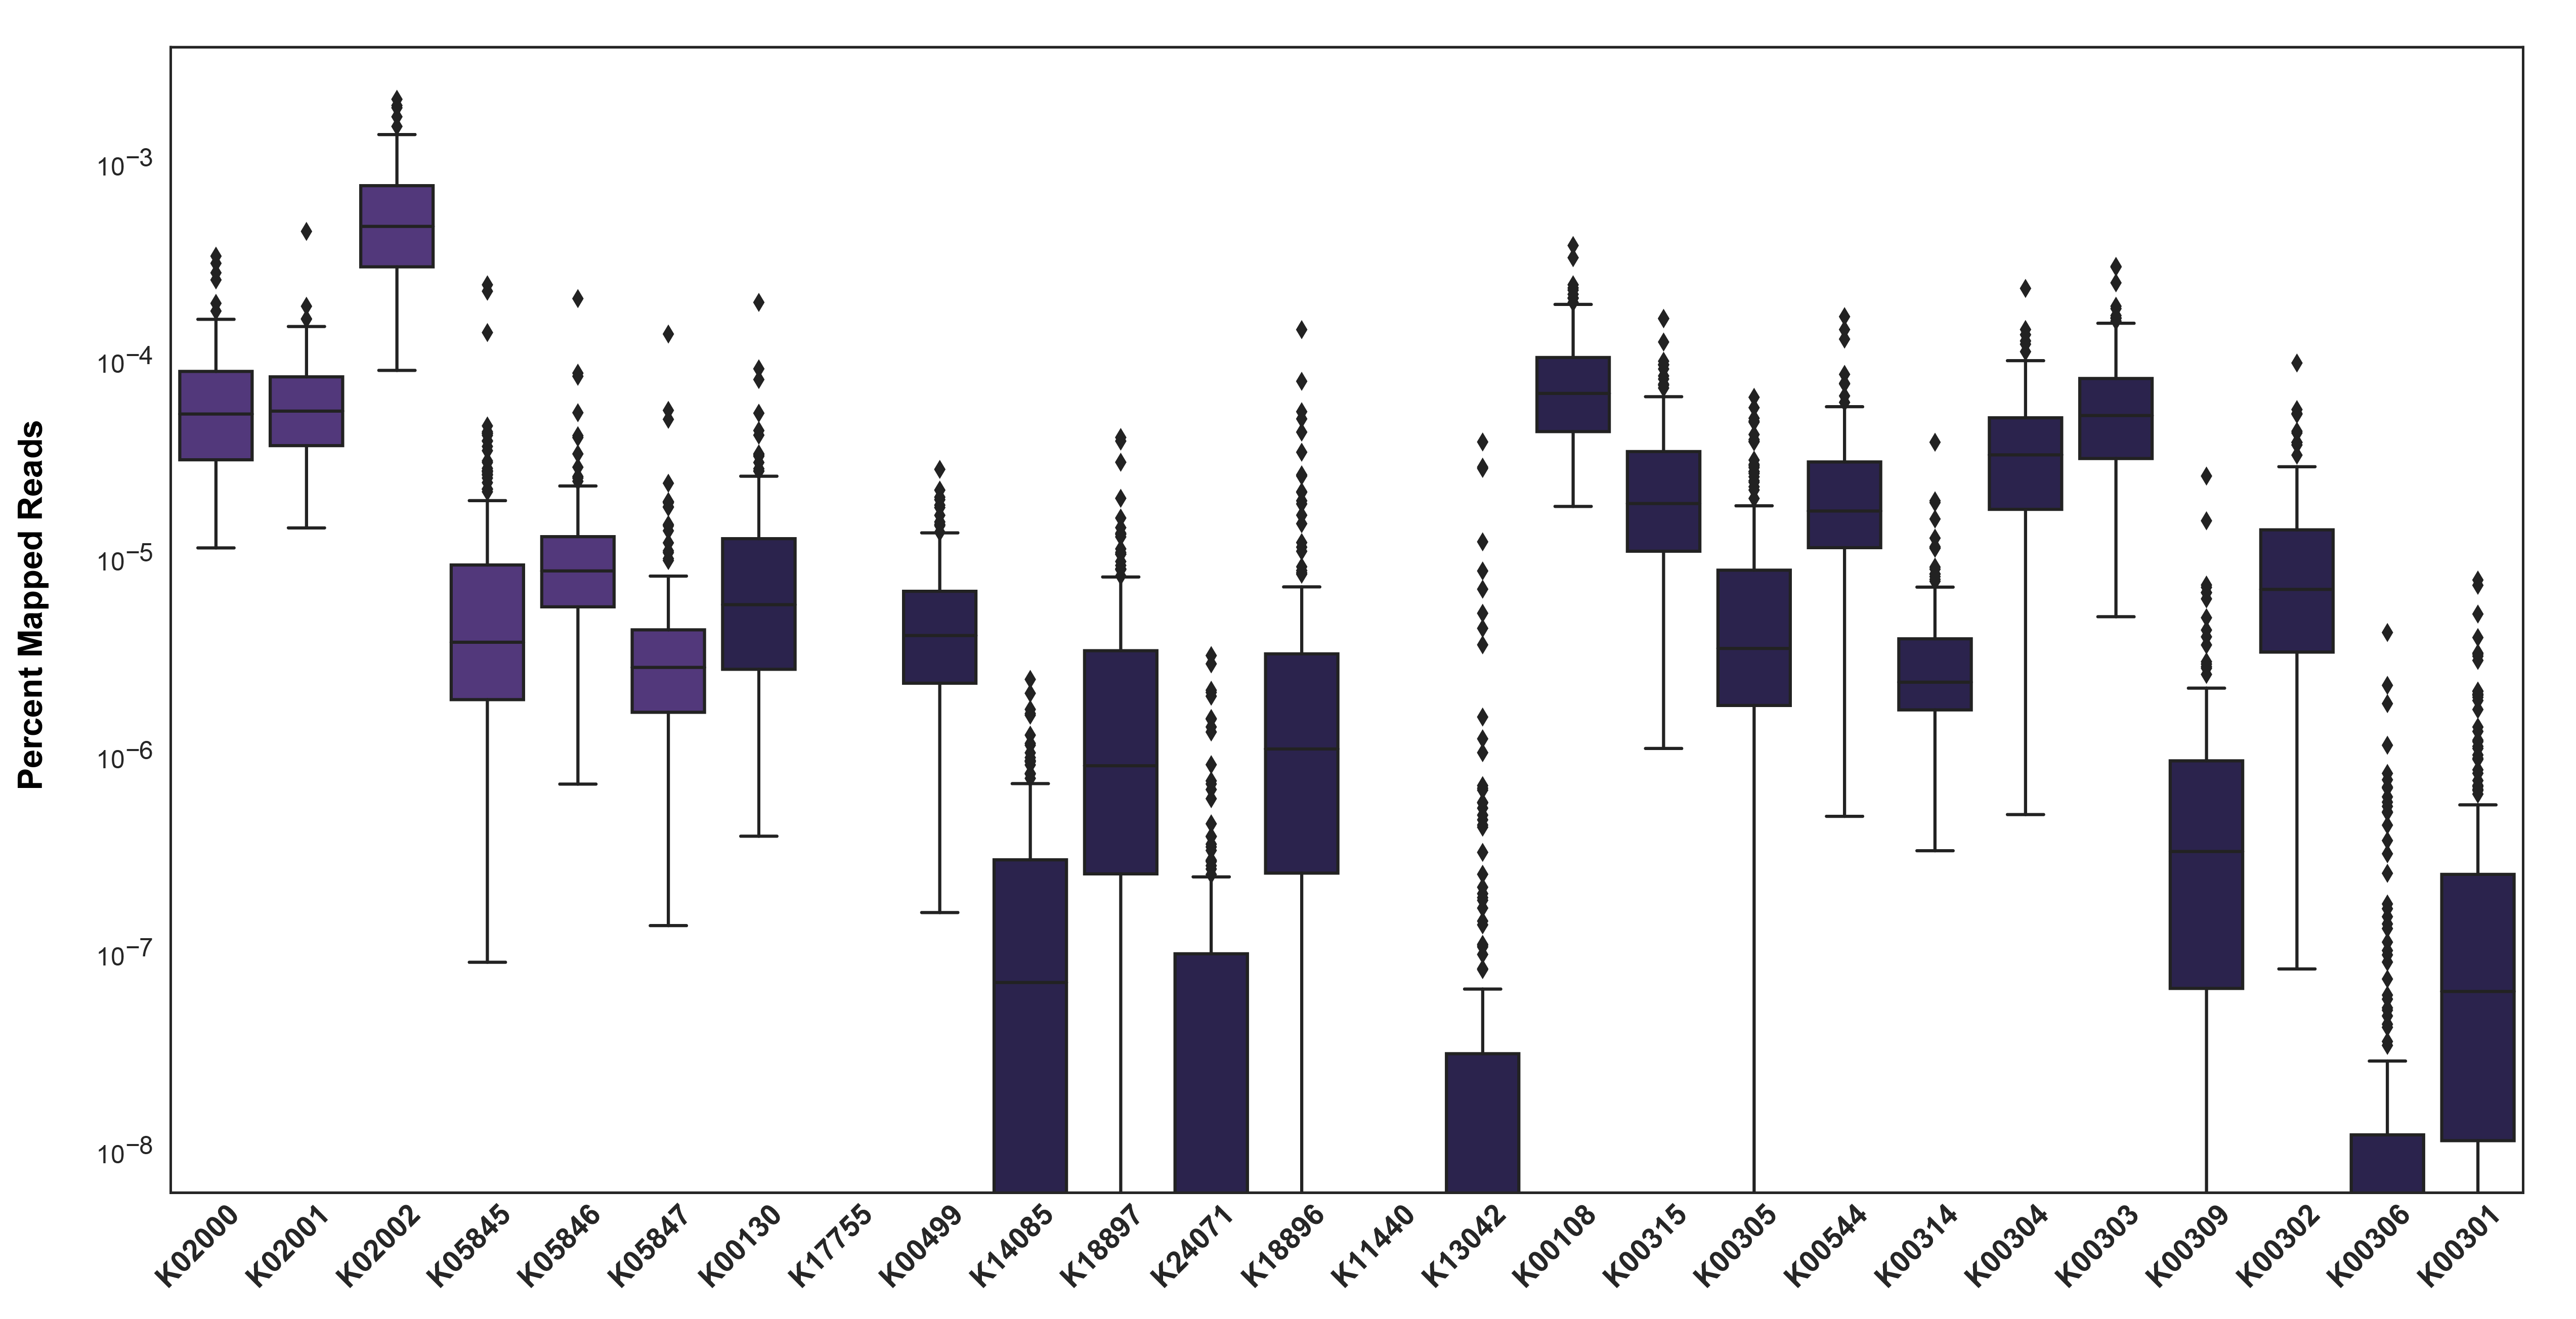
\includegraphics[width=0.9\columnwidth]{Figures/SI-Bact_Glycine_betaine_distributions-01.png}
    \caption{Prokaryotic metatranscriptome abundance of KEGG orthologs involved in the metabolism of glycine betaine.  The percent mapped read abundance of all orthologs recovered for each KO were summed by sample for the bacterial metatranscriptomic data from Tara Oceans using the OM-RGC v2 dataset. The distribution of all abundance data is shown as a box plot. Transporters are highlighted in light purple, synthesis and breakdown KOs are highlighted in dark purple.}
    \label{fig:bact-GB}
\end{figure*}

\begin{figure*}[ht]
    \centering
    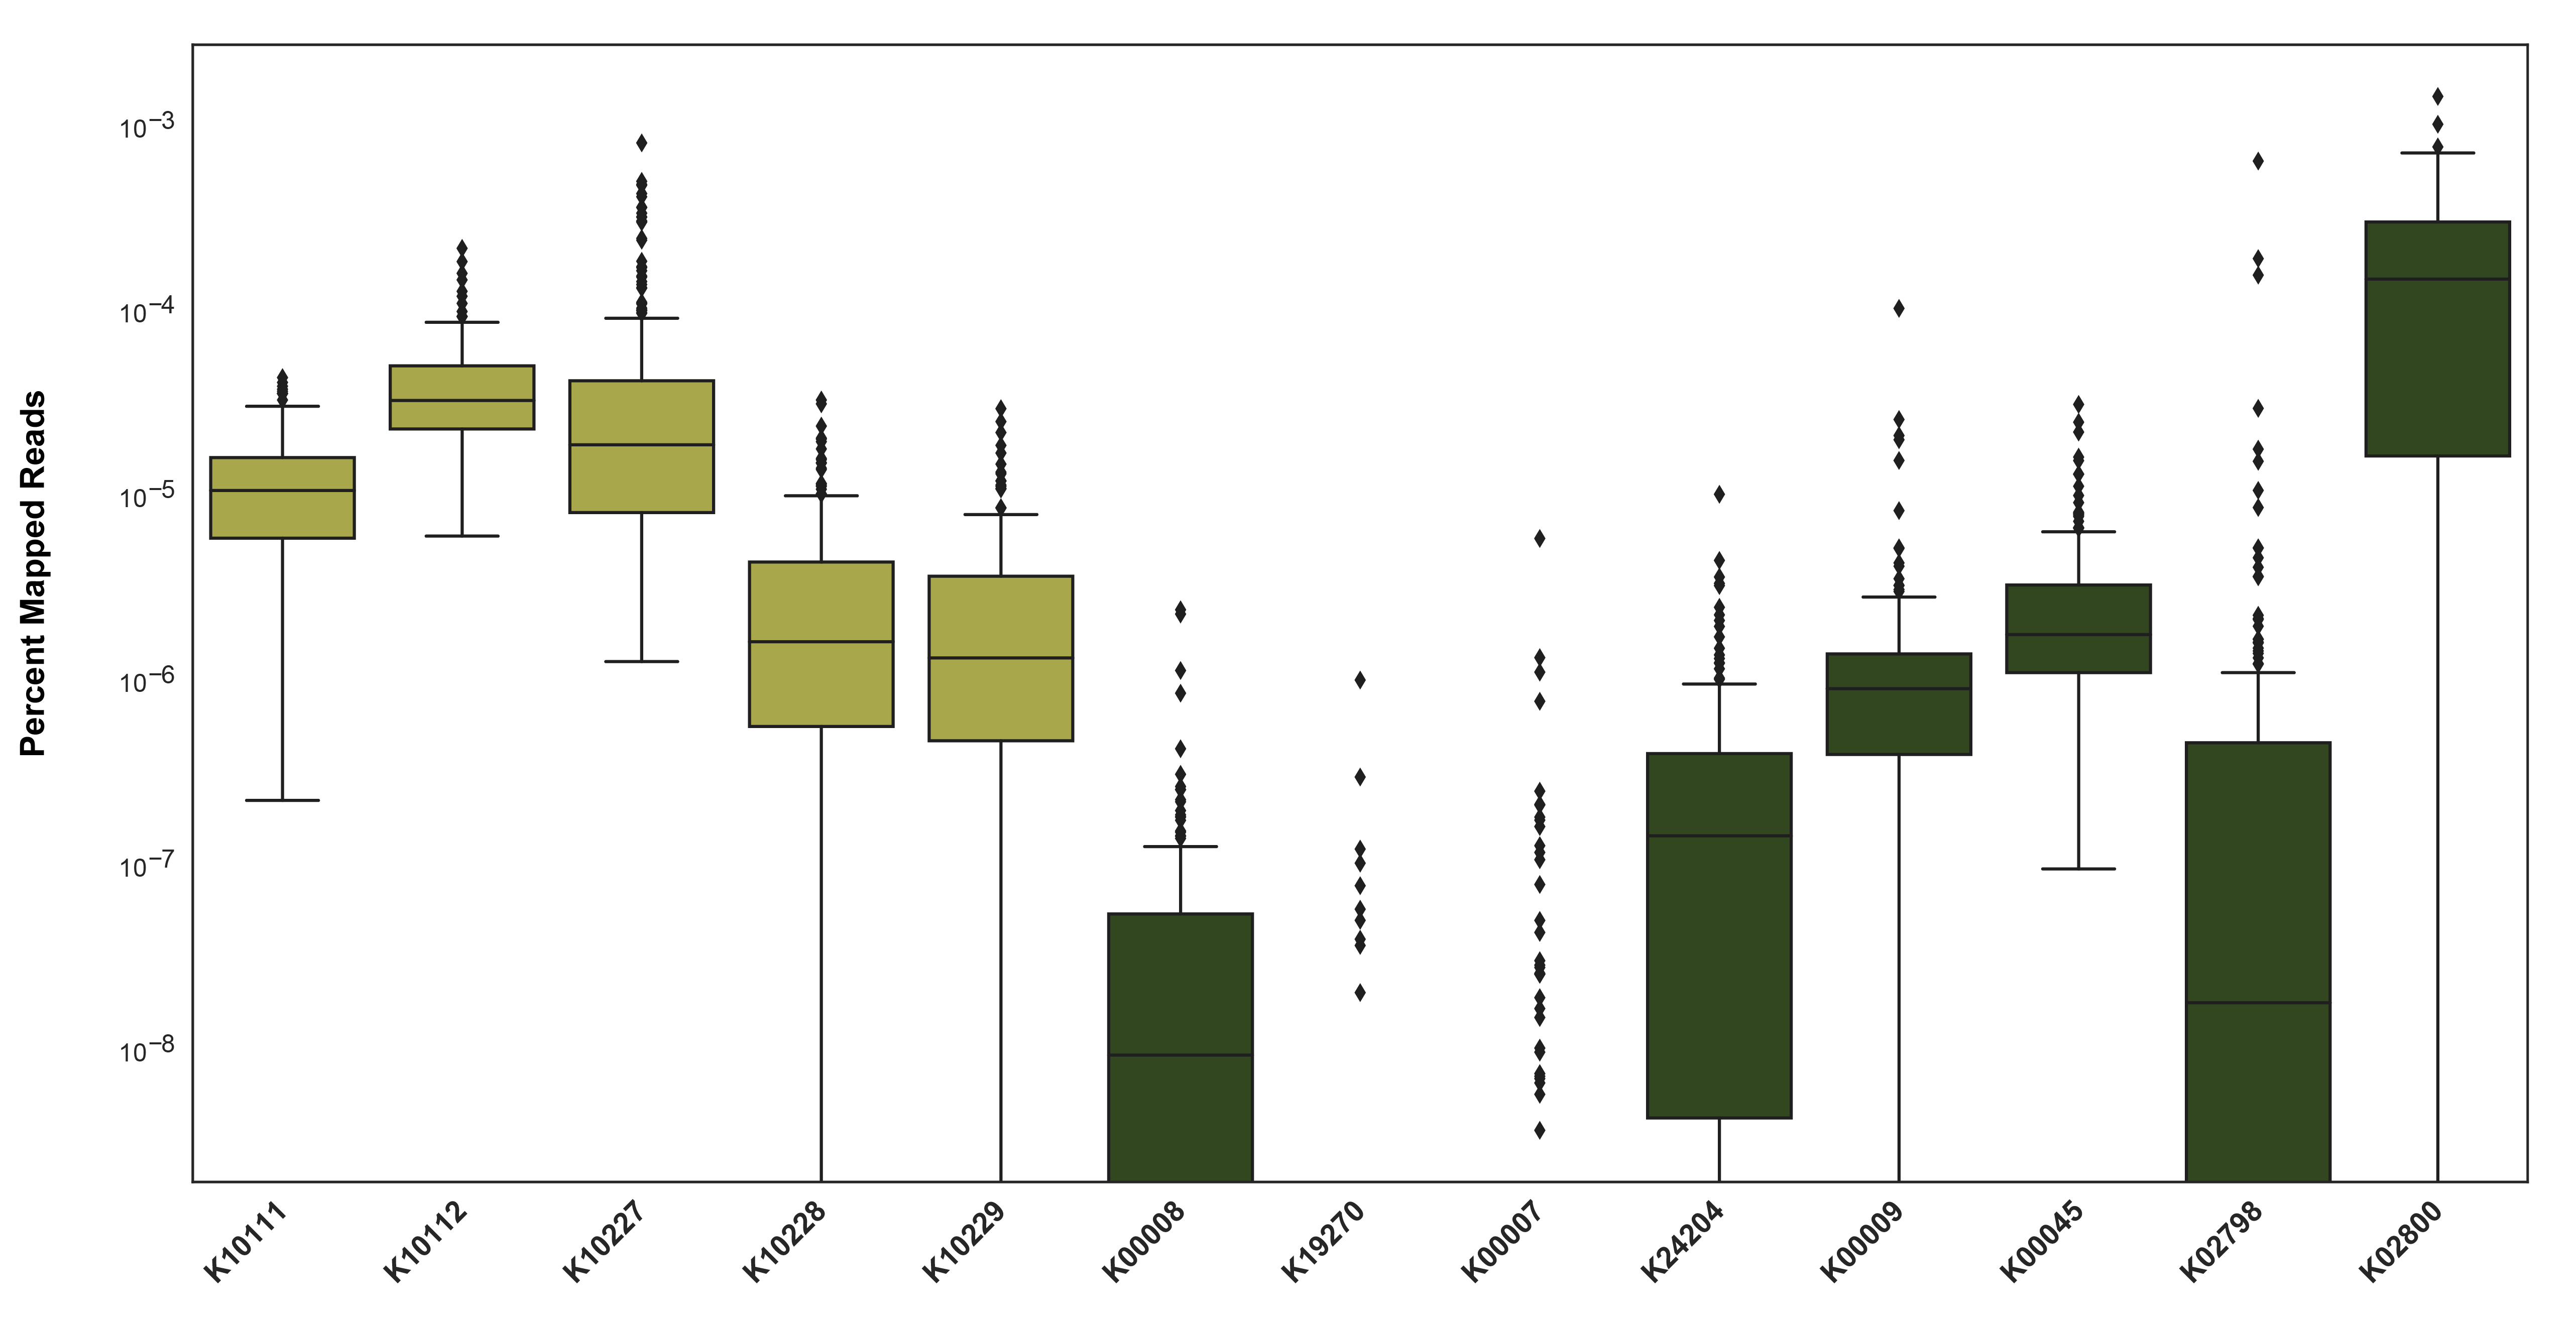
\includegraphics[width=0.9\columnwidth]{Figures/SI-Bact_Manitol_distributions-01.png}
    \caption{Prokaryotic metatranscriptome abundance of KEGG orthologs involved in the metabolism of mannitol.  The percent mapped read abundance of all orthologs recovered for each KO were summed by sample for the bacterial metatranscriptomic data from Tara Oceans using the OM-RGC\_v2 dataset. The distribution of all abundance data is shown as a box plot. Transporters are highlighted in light green, synthesis and breakdown KOs are highlighted in dark green.}
    \label{fig:bact-Man}
\end{figure*}

\begin{figure*}[ht]
    \centering
    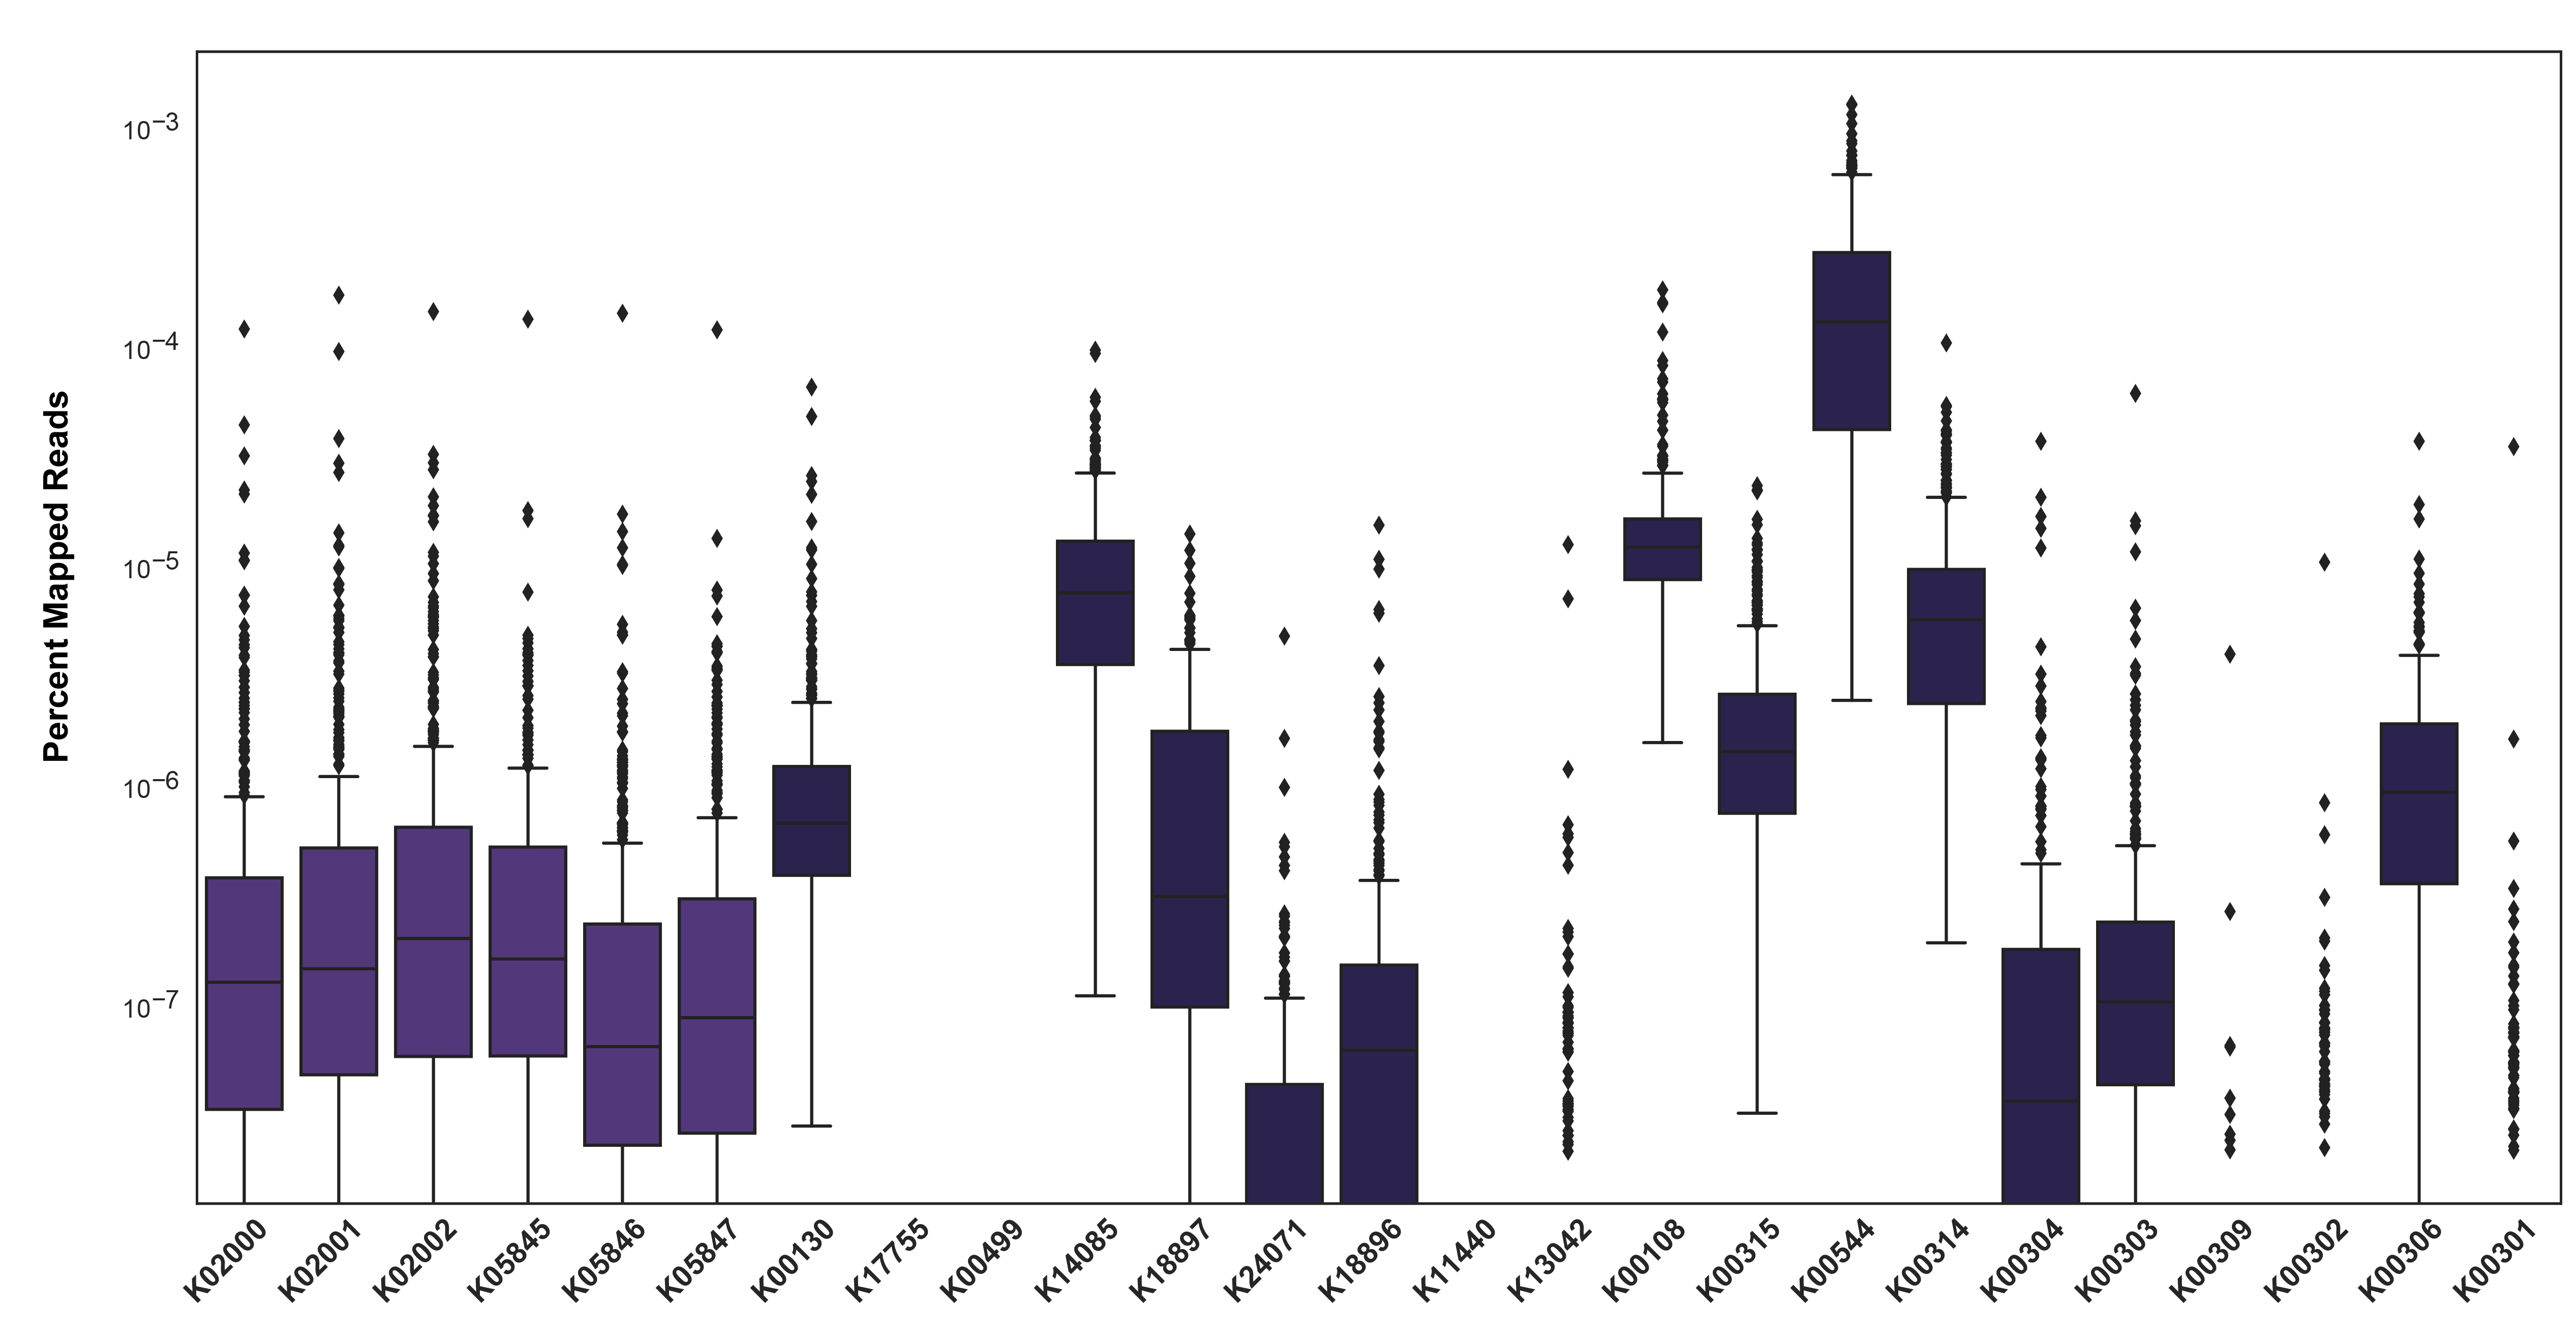
\includegraphics[width=0.9\columnwidth]{Figures/SI-Euk-Glycine_betaine_distributions-01.png}
    \caption{Eukaryotic metatranscriptome abundance of KEGG orthologs involved in the metabolism of glycine betaine.  The percent mapped read abundance of all orthologs recovered for each KO were summed by sample for the bacterial metatranscriptomic data from Tara Oceans using the MATOU-v1 dataset. The distribution of all abundance data is shown as a box plot. Transporters are highlighted in light purple, synthesis and breakdown KOs are highlighted in dark purple.}
    \label{fig:euk-GB}
\end{figure*}

\begin{figure*}[ht]
    \centering
    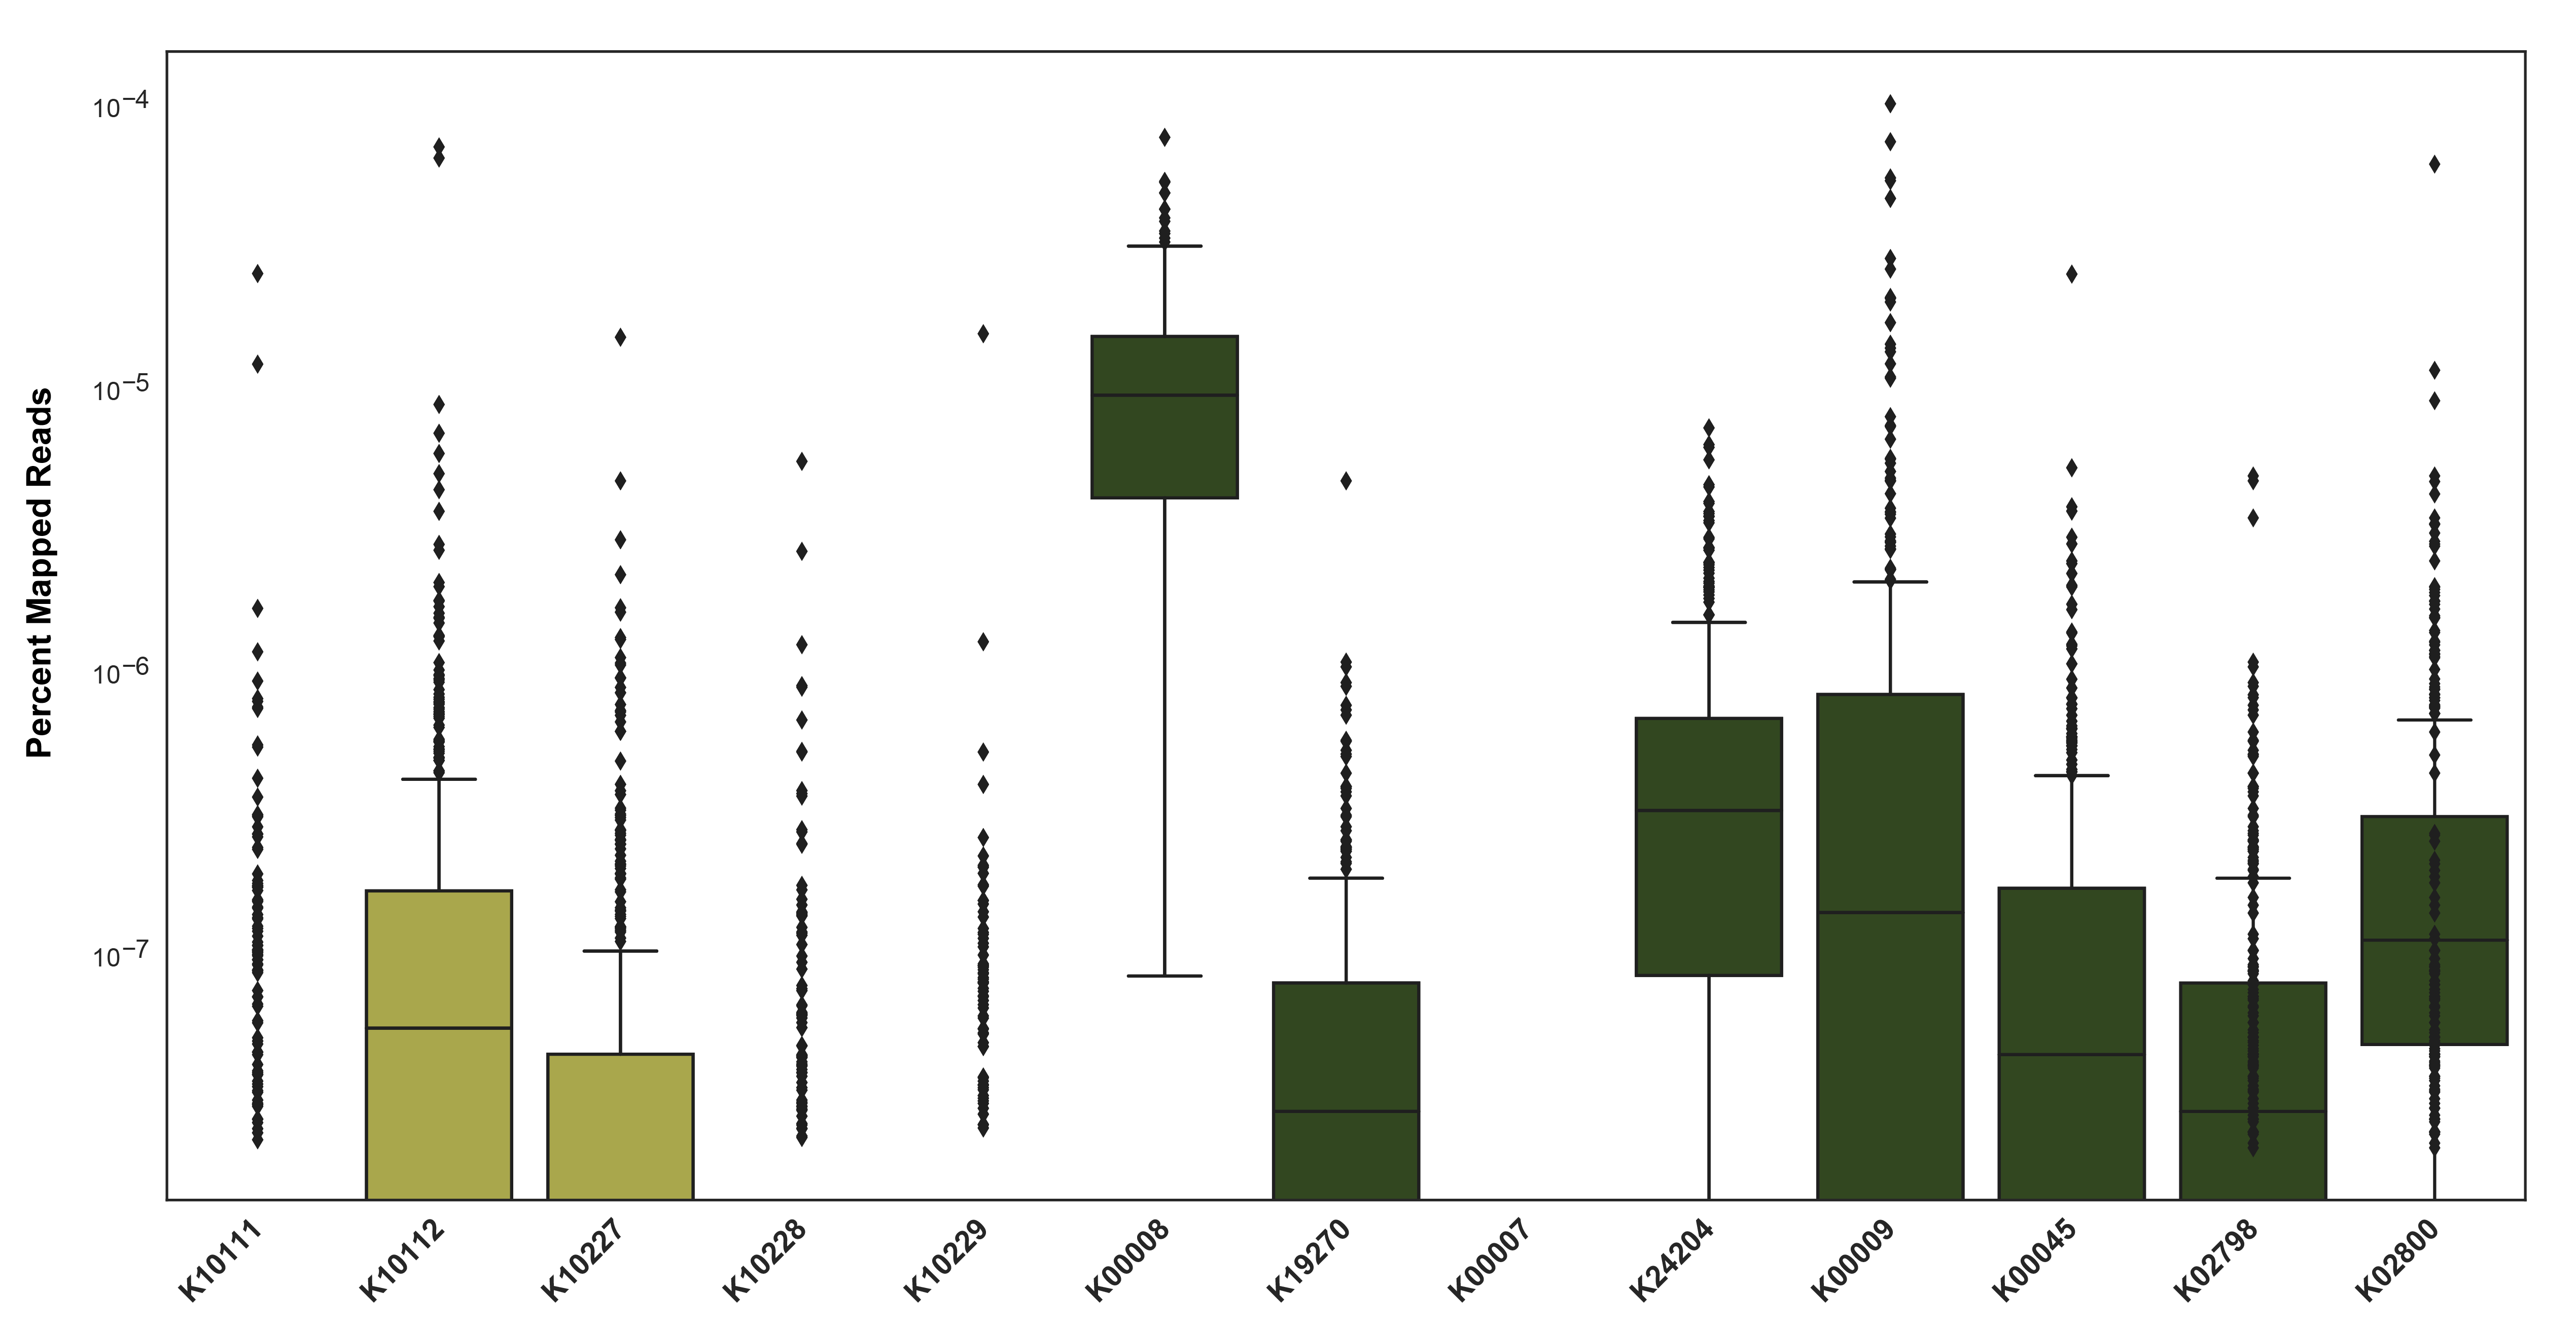
\includegraphics[width=0.9\columnwidth]{Figures/SI-Euk_Manitol_distributions-01.png}
    \caption{Eukaryotic metatranscriptome abundance of KEGG orthologs involved in the metabolism of mannitol.  The percent mapped read abundance of all orthologs recovered for each KO were summed by sample for the bacterial metatranscriptomic data from Tara Oceans using the MATOU-v1 dataset. The distribution of all abundance data is shown as a box plot. Transporters are highlighted in light green, synthesis and breakdown KOs are highlighted in dark green.}
    \label{fig:euk-Man}
\end{figure*}



\begin{figure*}[ht]
    \centering
    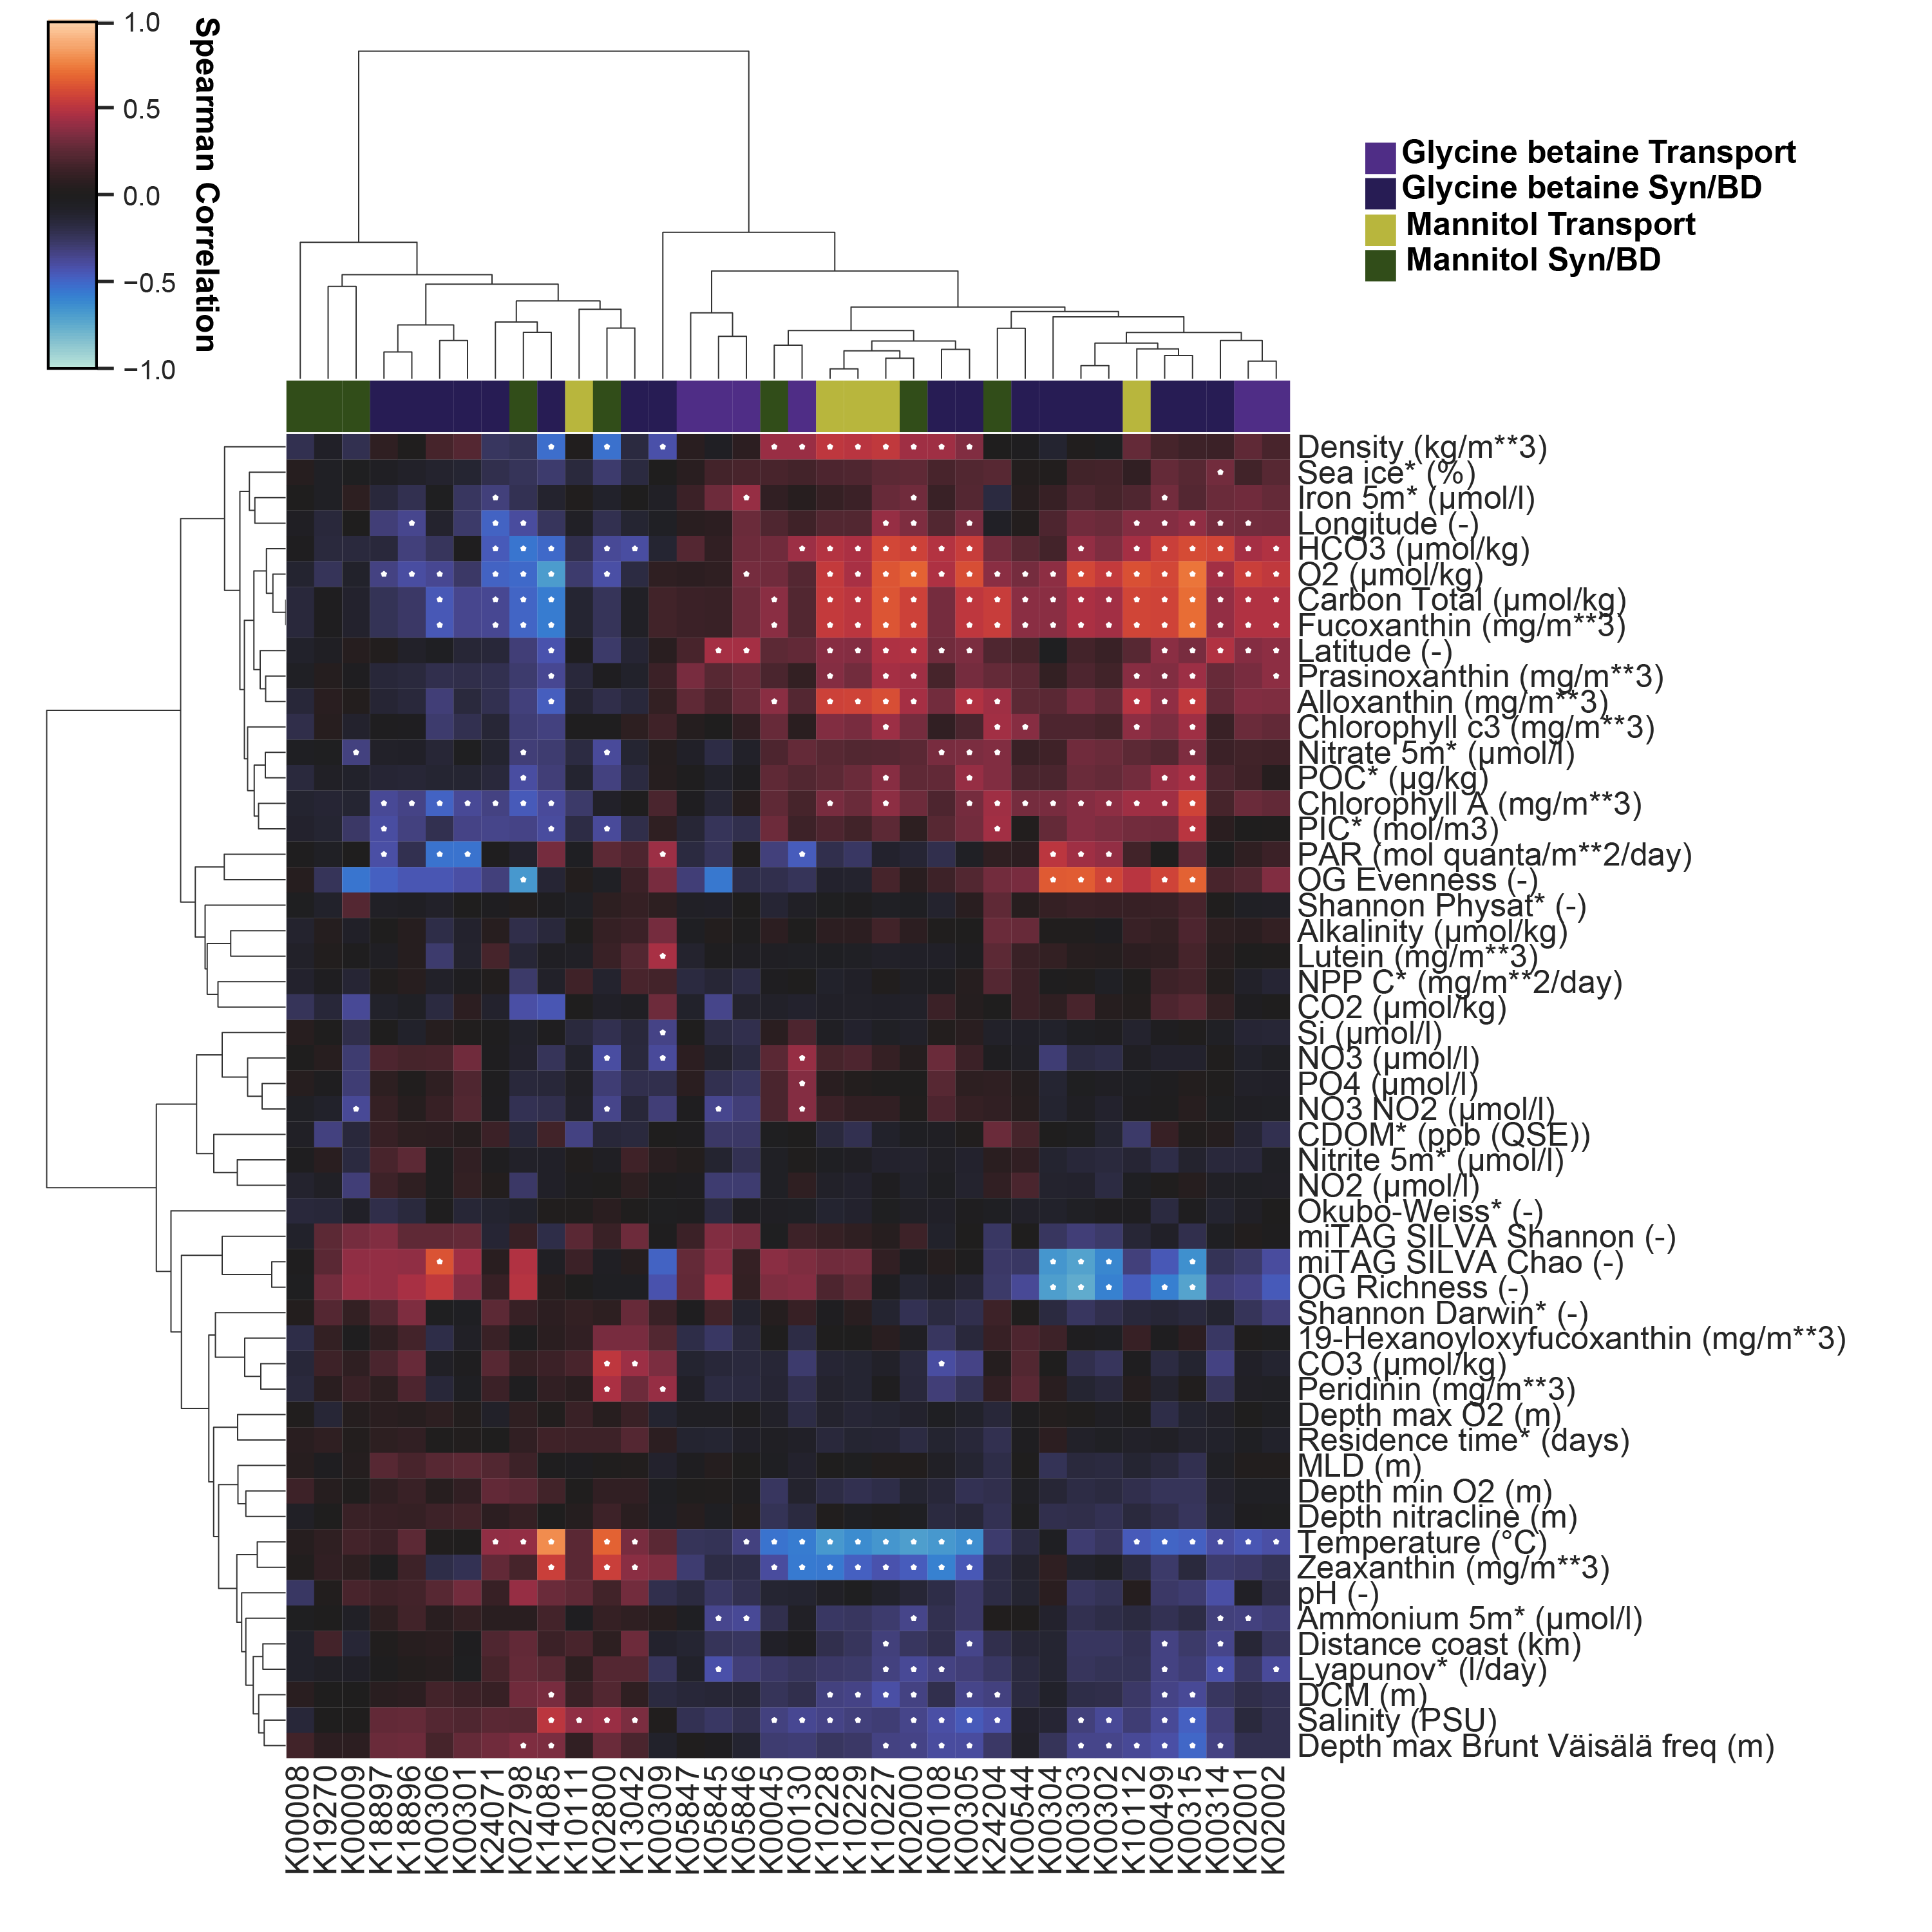
\includegraphics[width=0.9\columnwidth]{Figures/SI-bact_envfeature_spearman-01.png}
    \caption{Spearman correlation against environmental parameters from Tara. The global abundance of key orthologs involved in the synthesis, breakdown, and transport of mannitol (green) and glycine betaine (purple) from prokaryotic metatranscriptomic data from Tara was correlated with core environmental parameters. The metatranscriptomic abundance (percent mapped reads) of each of the orthologs involved in the processing of the osmolytes shown here was assessed across the bacterial metatranscriptomic data from Tara Oceans using the OM-RGC\_v2 dataset. The relative correlation of metatranscriptomic profiles for each of the orthologs considered was assessed by taking the Spearman's correlation of the sum of all orthologs associated with a KO at a given site and correlating it with available metadata. The Spearman's $\rho$ is depicted with a heatmap that is clustered based on Bray-Curtis similarity. Significant correlations were determined with a Bonferroni multi-testing p-value correction, and significant correlations ($p<0.001$) are depicted as a white dot.}
    \label{fig:bact-spearman}
\end{figure*}

\begin{figure*}[ht]
    \centering
    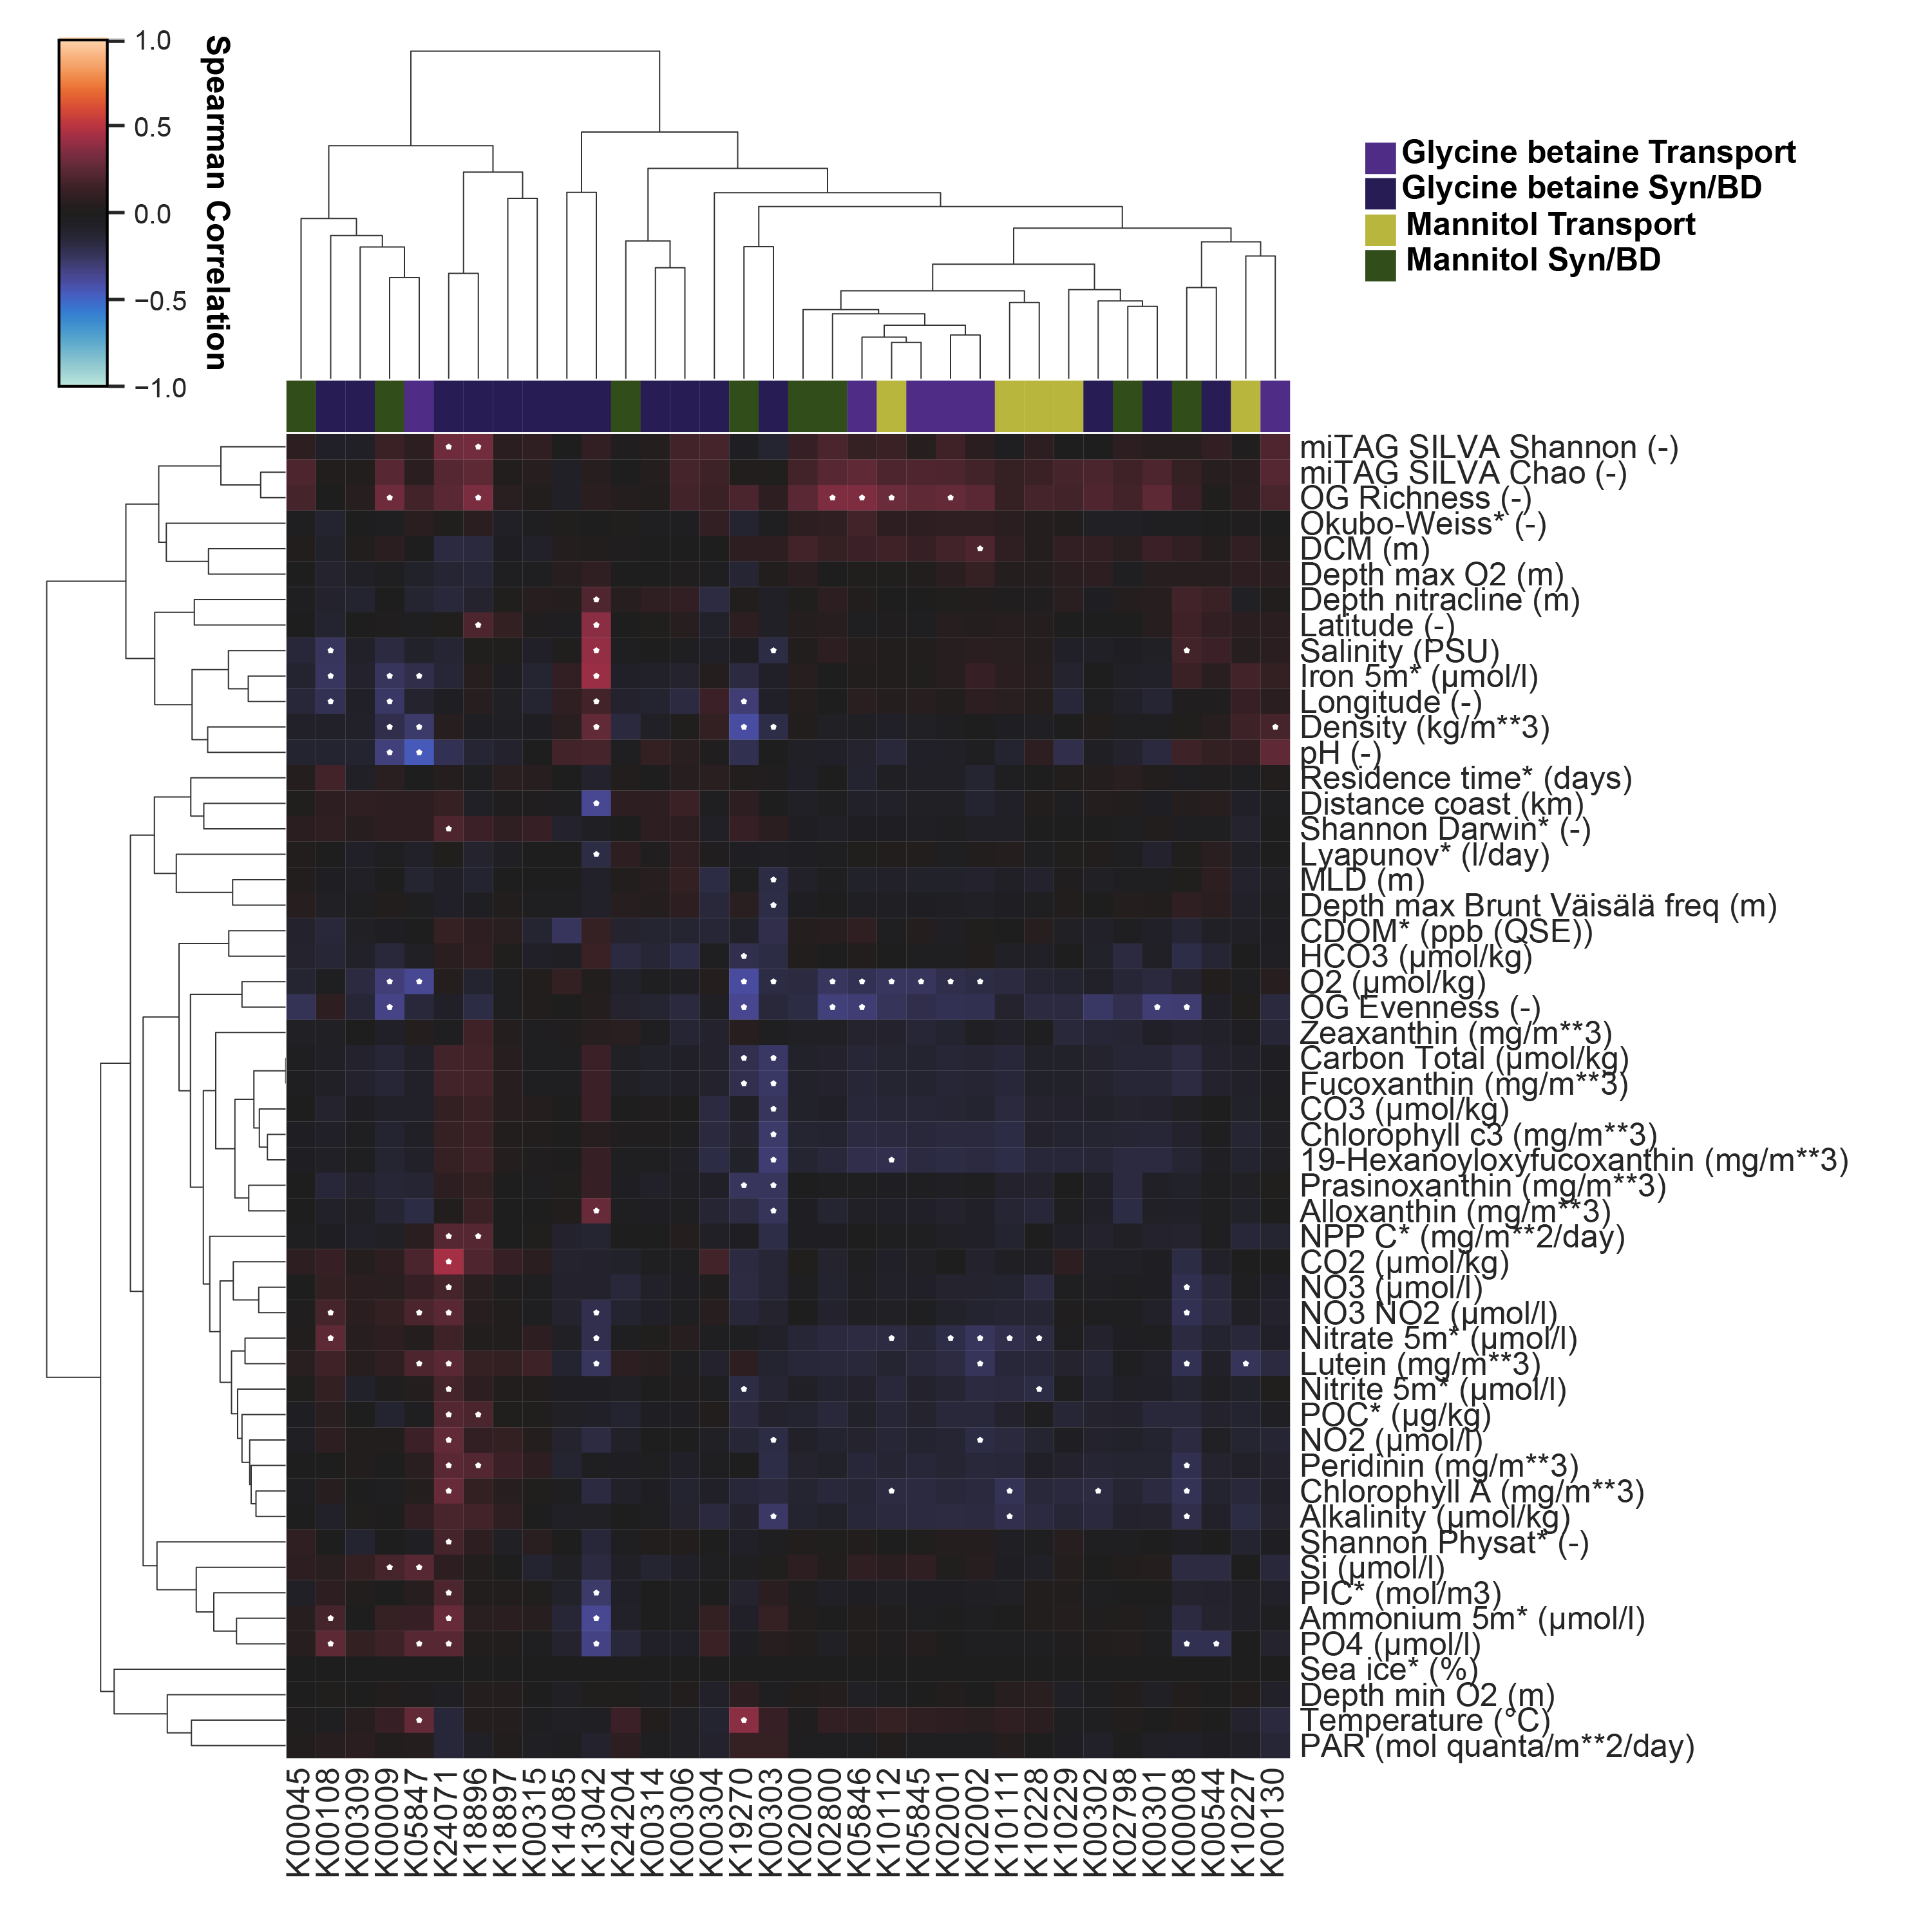
\includegraphics[width=0.9\columnwidth]{Figures/SI-euk_envfeature_spearman-01.png}
      \caption{Spearman correlation against environmental parameters from Tara. The global abundance of key orthologs involved in the synthesis, breakdown, and transport of mannitol (green) and glycine betaine (purple) from eukaryotic metatranscriptomic data from Tara was correlated with core environmental parameters. The metatranscriptomic abundance (percent mapped reads) of each of the orthologs involved in the processing of the osmolytes shown here was assessed across the bacterial metatranscriptomic data from Tara Oceans using the MATOU-v1 dataset. The relative correlation of metatranscriptomic profiles for each of the orthologs considered was assessed by taking the Spearman's correlation of the sum of all orthologs associated with a KO at a given site and correlating it with available metadata. The Spearman's $\rho$ is depicted with a heatmap that is clustered based on Bray-Curtis similarity. Significant correlations were determined with a Bonferroni multi-testing p-value correction, and significant correlations ($p<0.001$) are depicted as a white dot.}
    \label{fig:euk-spearman}
\end{figure*}
%%% There is no need for adding the file termination, as long as you indicate where the file is saved. In the examples below the files (logo1.eps and logos.eps) are in the Frontiers LaTeX folder
%%% If using *.tif files convert them to .jpg or .png
%%%  NB logo1.eps is required in the path in order to correctly compile front page header %%%



\end{document}

